\documentclass{article}
\usepackage{graphicx}
\usepackage[top=.5in,bottom=.5in,right=.5in,left=.5in]{geometry}
\usepackage{hyperref}
\begin{document}
\title{QSFP+ Fiber Optic Tests}
\author{Zuhra Abdurashidova and Jack Hickish}
\maketitle


%Add qsfp explanation, what 40Gbe really means, speed of data transmission, explanation about packet size, amount of packet transmissions, 

\section*{Introduction}

Hydrogen Epoch of Reionization Array will probe deeper than ever into the mysteries of early star and galaxy formation. The array will be comprised of 352 dishes located in the South African Karoo desert.  The data from dishes will be digitized at nodes close to the array and sent for correlation and processing to the Karoo Array Processor Building a few kilometers away. The required data rate for HERA is around 10 Gbps. Considering the number of dishes, fast data rate and remote location, fiber optic technology offers a cheap, fast and reliable data transmission from dishes to correlator. 

SNAP boards located at various boxes (nodes) throughout the array are responsible for digitizing the signal and transmitting it along a fiber back to KAPB. Each node contains four SNAP boards. Each SNAP board processes a signal from three antennas at a rate of 10 Gbps. This results in 352/3 =118 fiber optic cables running from the array to KAPB where correlation takes place. In an effort to reduce the cost and amount of fiber involved, multiplexor technology will be implemented. Multiplexors (also called muxes) combine multiple signals onto a single fiber using a diffraction grating. Provided that each SNAP board in a node uses a unique wavelength transceiver, it is possible to multiplex the four signals onto a single fiber, thus reducing the amount of fibers necessary by four. It is possible to multiplex more than four signals onto one fiber. CWDM-18 ( Course Wave Division Multiplexing of 18 signals) and CWDM-44 technologies are readily available but would make signal processing more complicated. For example, having 18 signals on one line would require bigger,more complicated switches with a huge amount of SFP+ ports. With CWDM-4 we can use QSFP+ transceivers that are made specifically for 4 laser inputs and attach to less complex, QSFP+ switches. Also, using CWDM-4 and QSFP+ transceivers will make it easier to track fibers coming from various nodes since each node will have exactly one QSFP+ transceiver at the switch. 

The use of fiber introduces a problem of attenuation. The intensity of a signal decreases the longer it travels. This is caused by scattering of light due to imperfections in the fiber, conversion of some of its energy into heat, absorption and imperfect nature of connection points.  In order to make sure that the signals from dishes do not attenuate beyond the point of recognition by the transceiver, tests were carried out to determine the 'link margin' . Link margin tests provide the maximum attenuation value that could be reached before the onset of packet loss.  Transceivers send signals in the form of packets using UDP (User Datagram Protocol). Each packet has a header and the data itself. The header contains information like source/destination ports, length of data and error checking for the header and data. Packets get dropped when the attenuation in the fiber is above the link margin and transceiver is unable to pick up the information contained in the signal. The following tests probe to see if the attenuation due to fiber length and various connection points will be below the threshold at which packet loss occurs. 



\section*{The Basics}
There are probably certain aspects of these experiments that the interested reader is not quiet familiar with. This section will contain some basic definitions.
\begin{itemize}
\item Transceiver-A transceiver in this case is any network device that can both receive and transmit a signal. Transceivers come in different shapes and sizes and the choice for this experiment were the FiberStore CSFP (SFP+) 10Gb 20 km single mode transceivers that support 1270nm, 1290nm, 1310m and 1330nm wavelengths. CSFP stands for Compact Small Form-factor Pluggable transceiver. Transceivers are wideband and thus could receive any wavelength between 1260nm and 1620nm. However, each transceiver transmits only at the specified wavelength. FiberStore 40G 10km QSFP+ LR4 single mode transceivers were placed at the switch end and are able to process a muxed signal coming from four SFP+ transceivers.  
\item Multiplexer - A multiplexer is a device that can split (demux) a signal into its constituent parts via a diffraction grating or combine (mux) multiple signals into one. We used the CWDM (Coarse Wave Division Multiplexer) Mux/Demux pair. A multiplexer is a passive device. 
\item Attenuator - In order to model attenuation we introduced a variable attenuator into the signal chain. 
\item Long Distance Network Simulation Test Box (LDNSTB) - This is box of10km spool of fiber optic cable. It provides an attenuation of about 5.6dB. This serves as a benchmark for our tests since the correlator is a few kilometers away from SFP+ transceivers on the SNAP boards. 
\item LC connector - The type of connector used in the fiber optic cables. LC to FC was used to connect to the variable attenuator. Transceivers already come with LC connectors. All of the cables used in these experiments are single mode.  
\item Adapters - LC Adapters were used to connect various patches of LC cables (i.e. transceiver LC to Mux/Demux, Mux COM to QSFP LC etc). 
\end{itemize}

\begin{center}
\begin{tabular}{|l|p{2.5cm}|}
	\hline
	Transceiver color & Wavelength(nm)\\ \hline
	pink & 1270\\ \hline
	blue & 1290\\ \hline
	yellow & 1330\\ \hline
	green & 1310\\ \hline
\end{tabular}	
\end{center}


\begin{figure}[h]
\centering
	\begin{minipage}{.4\textwidth}
		\centering
		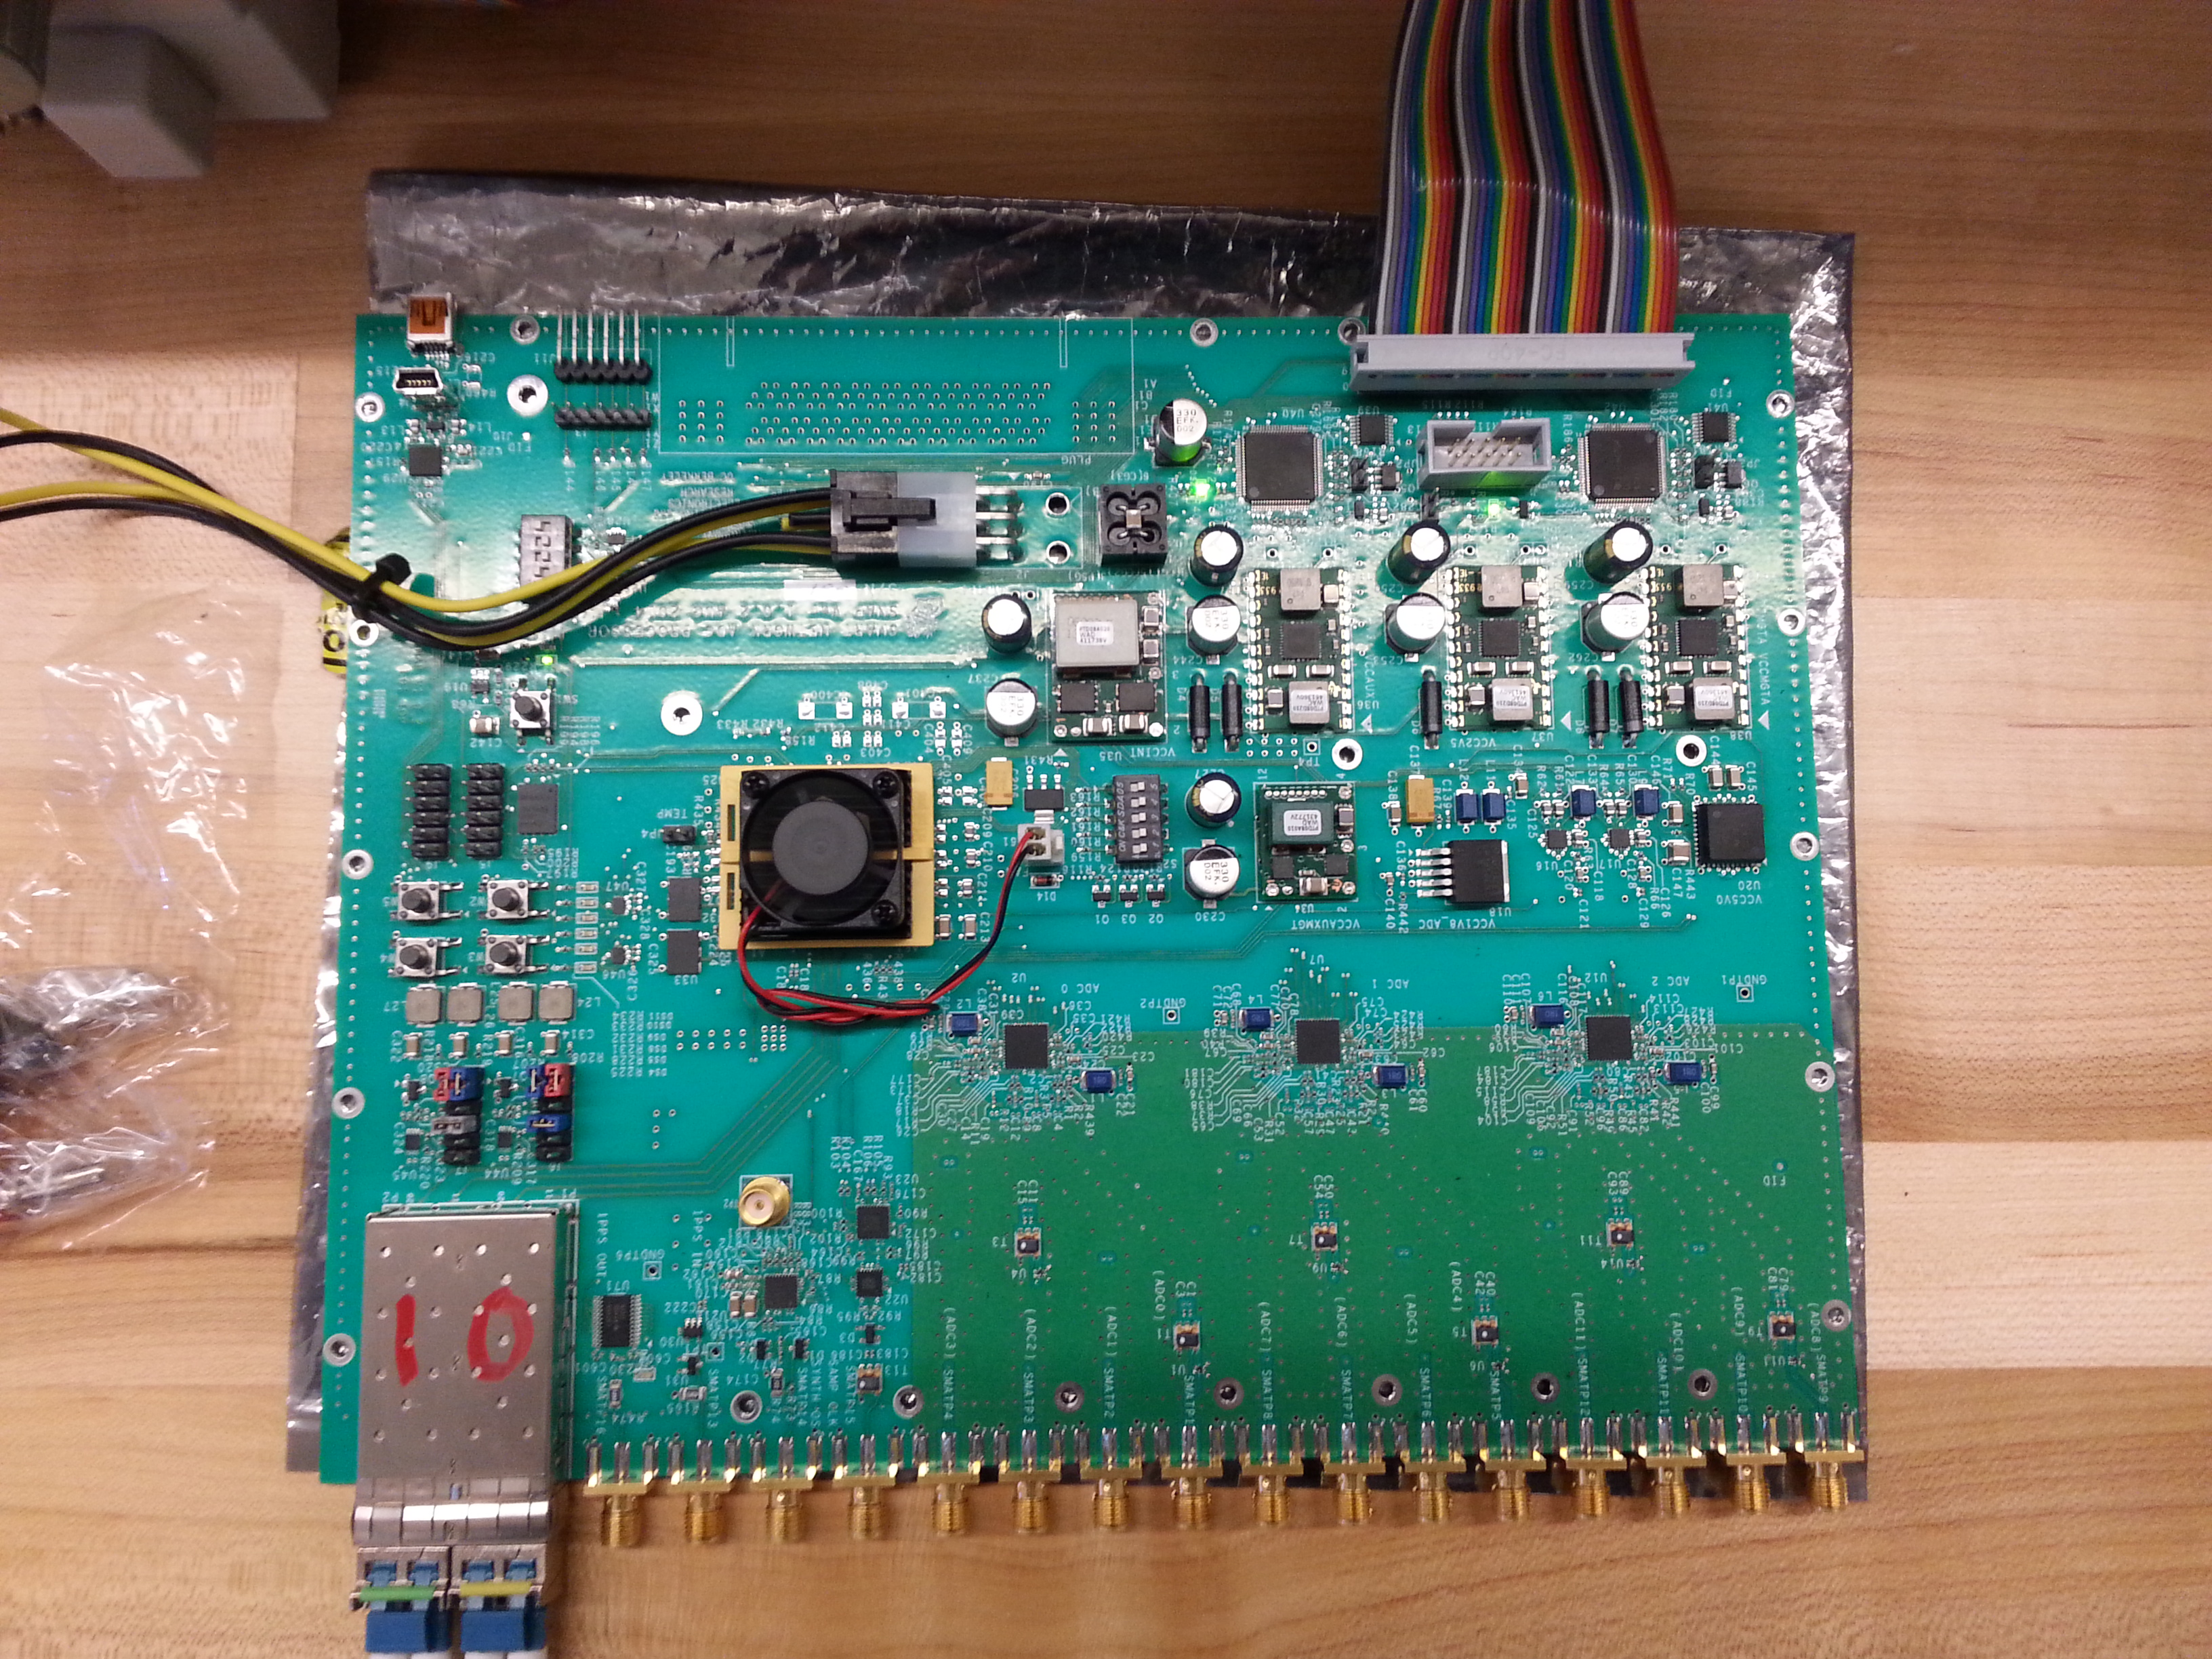
\includegraphics[width =.8\linewidth,height=2.6in]{SNAP.png}
		\caption{SNAP board of S/N: 001} 
	\end{minipage}
	\begin{minipage}{.4\textwidth}
		\centering
		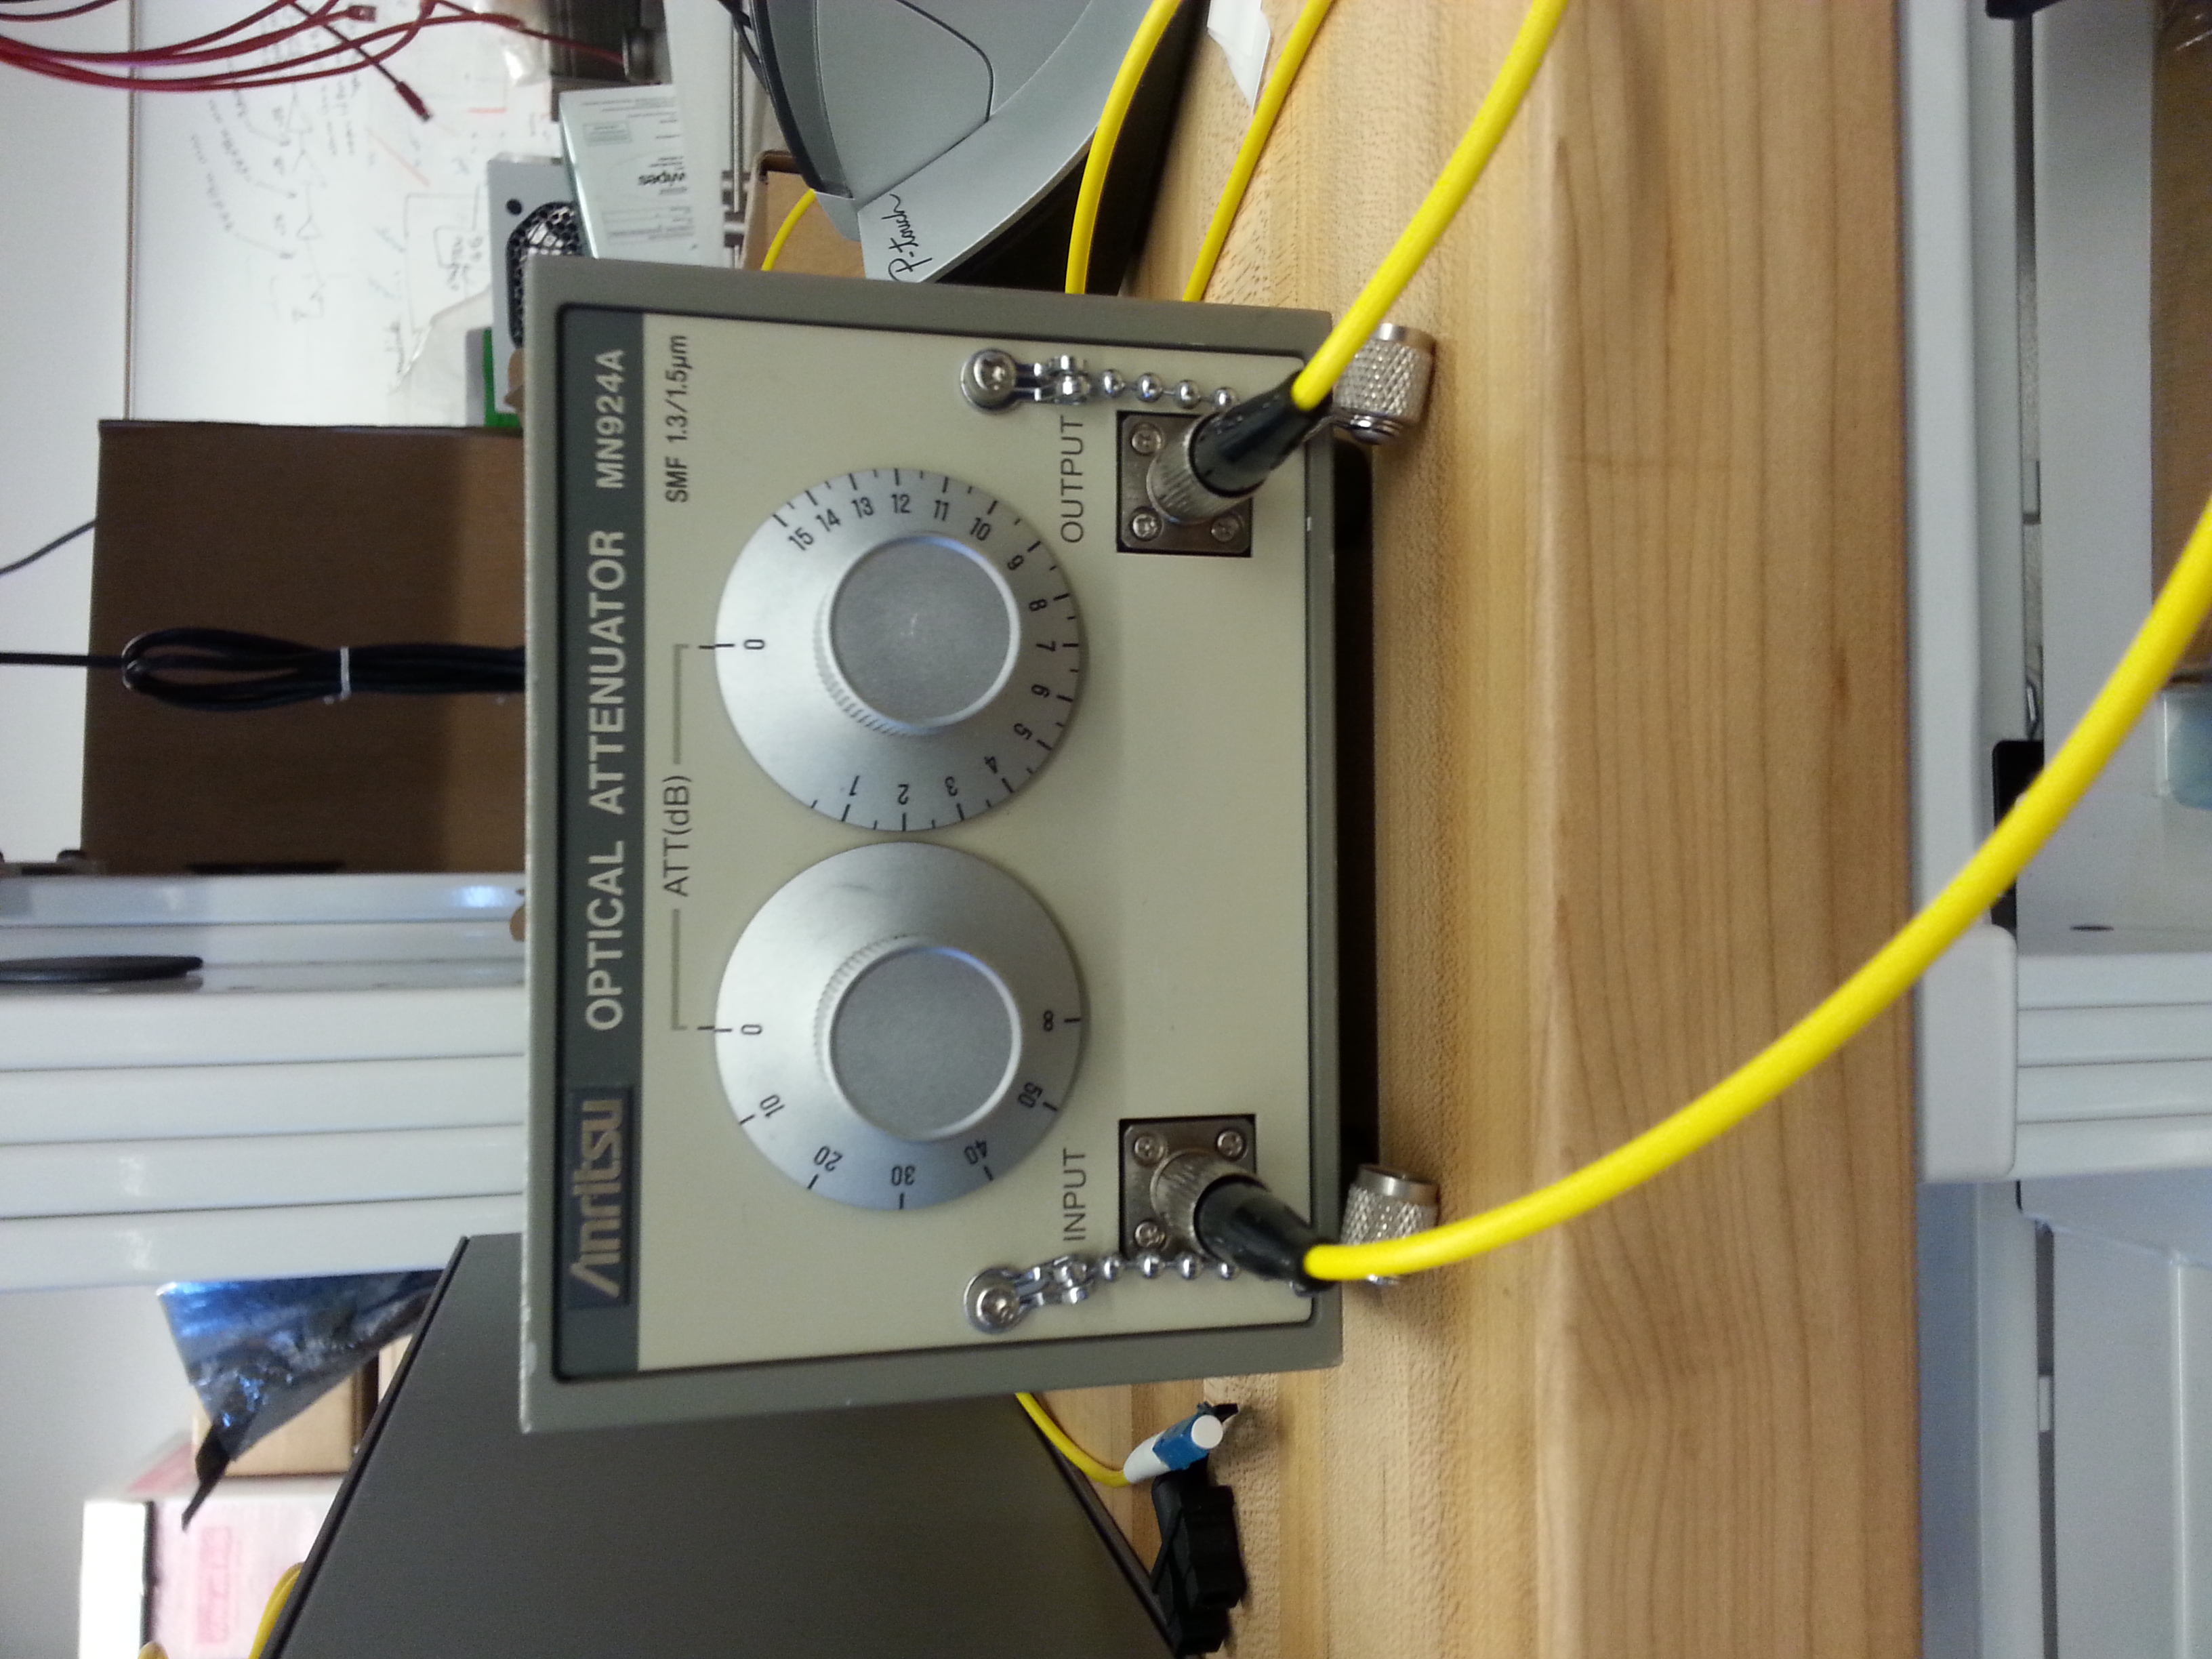
\includegraphics[width = .8\linewidth,height=2.6in]{att.png}
		\caption{Optical Attenuator}
	\end{minipage}
\end{figure}

\begin{figure}[h]
\centering
	\begin{minipage}{.4\textwidth}
		\centering
		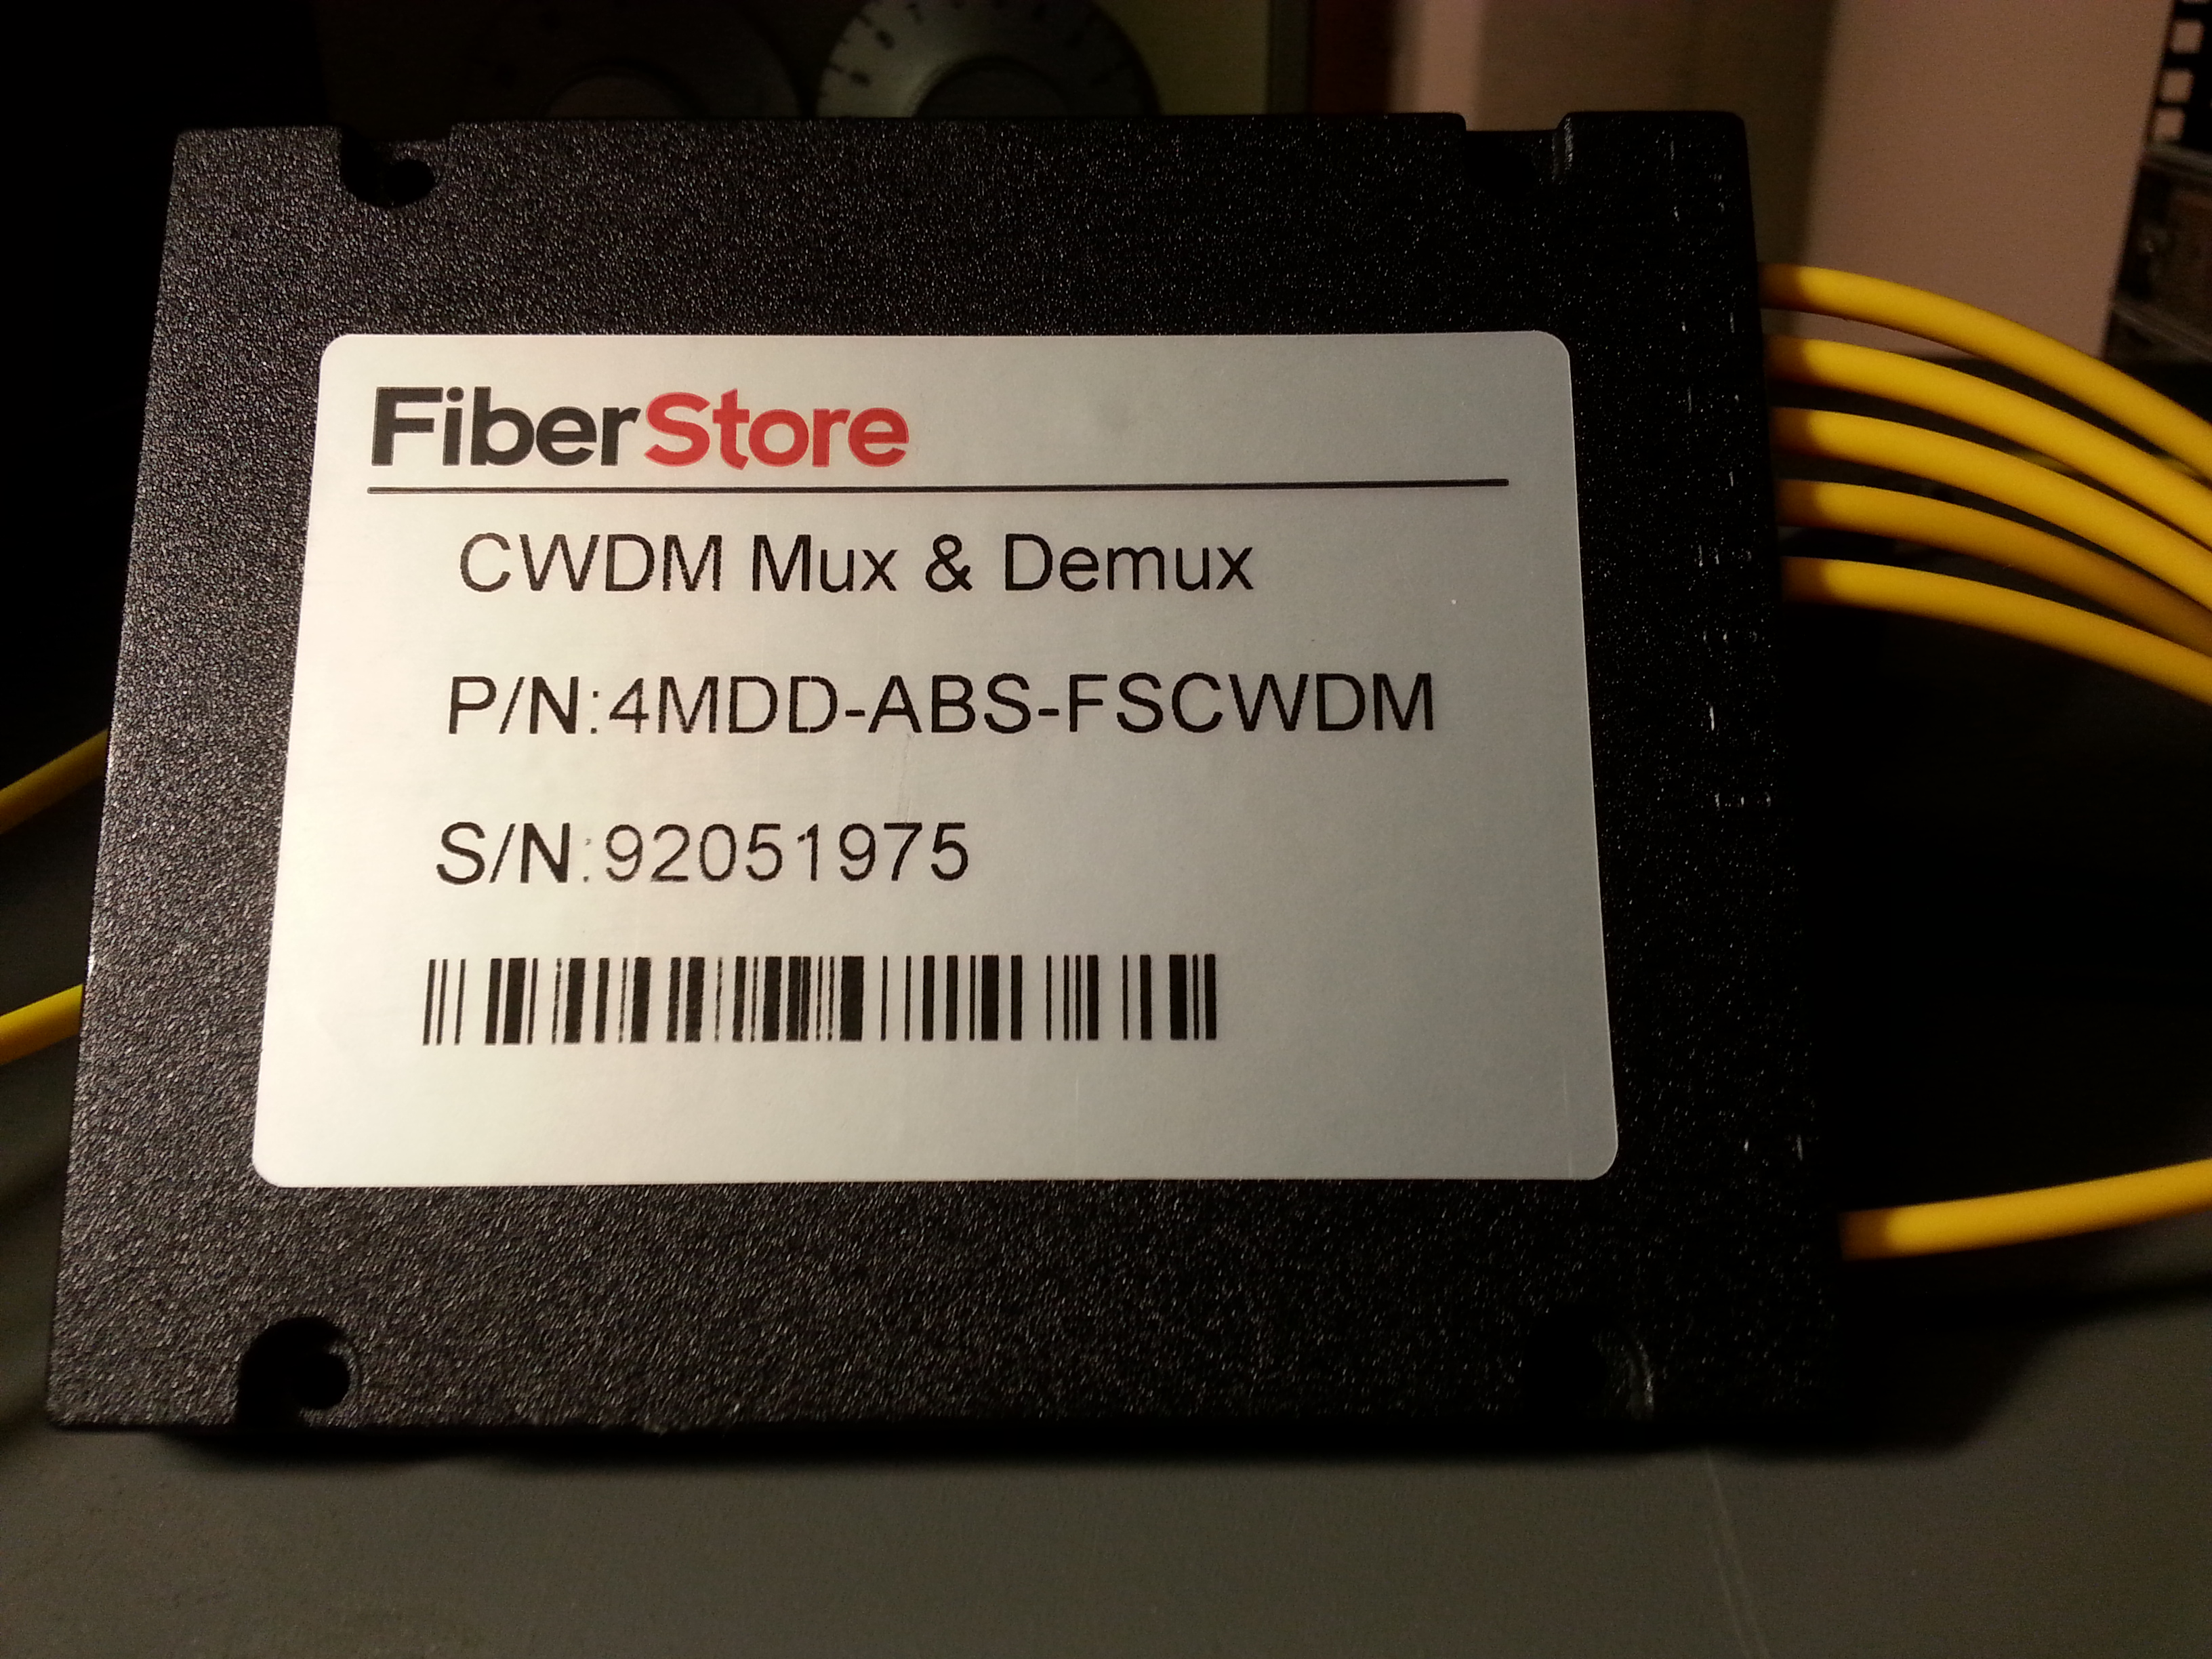
\includegraphics[width = .8\linewidth]{mux.jpg}
		\caption{Mux/Demux}
	\end{minipage}
	\begin{minipage}{.4\textwidth}
		\centering
		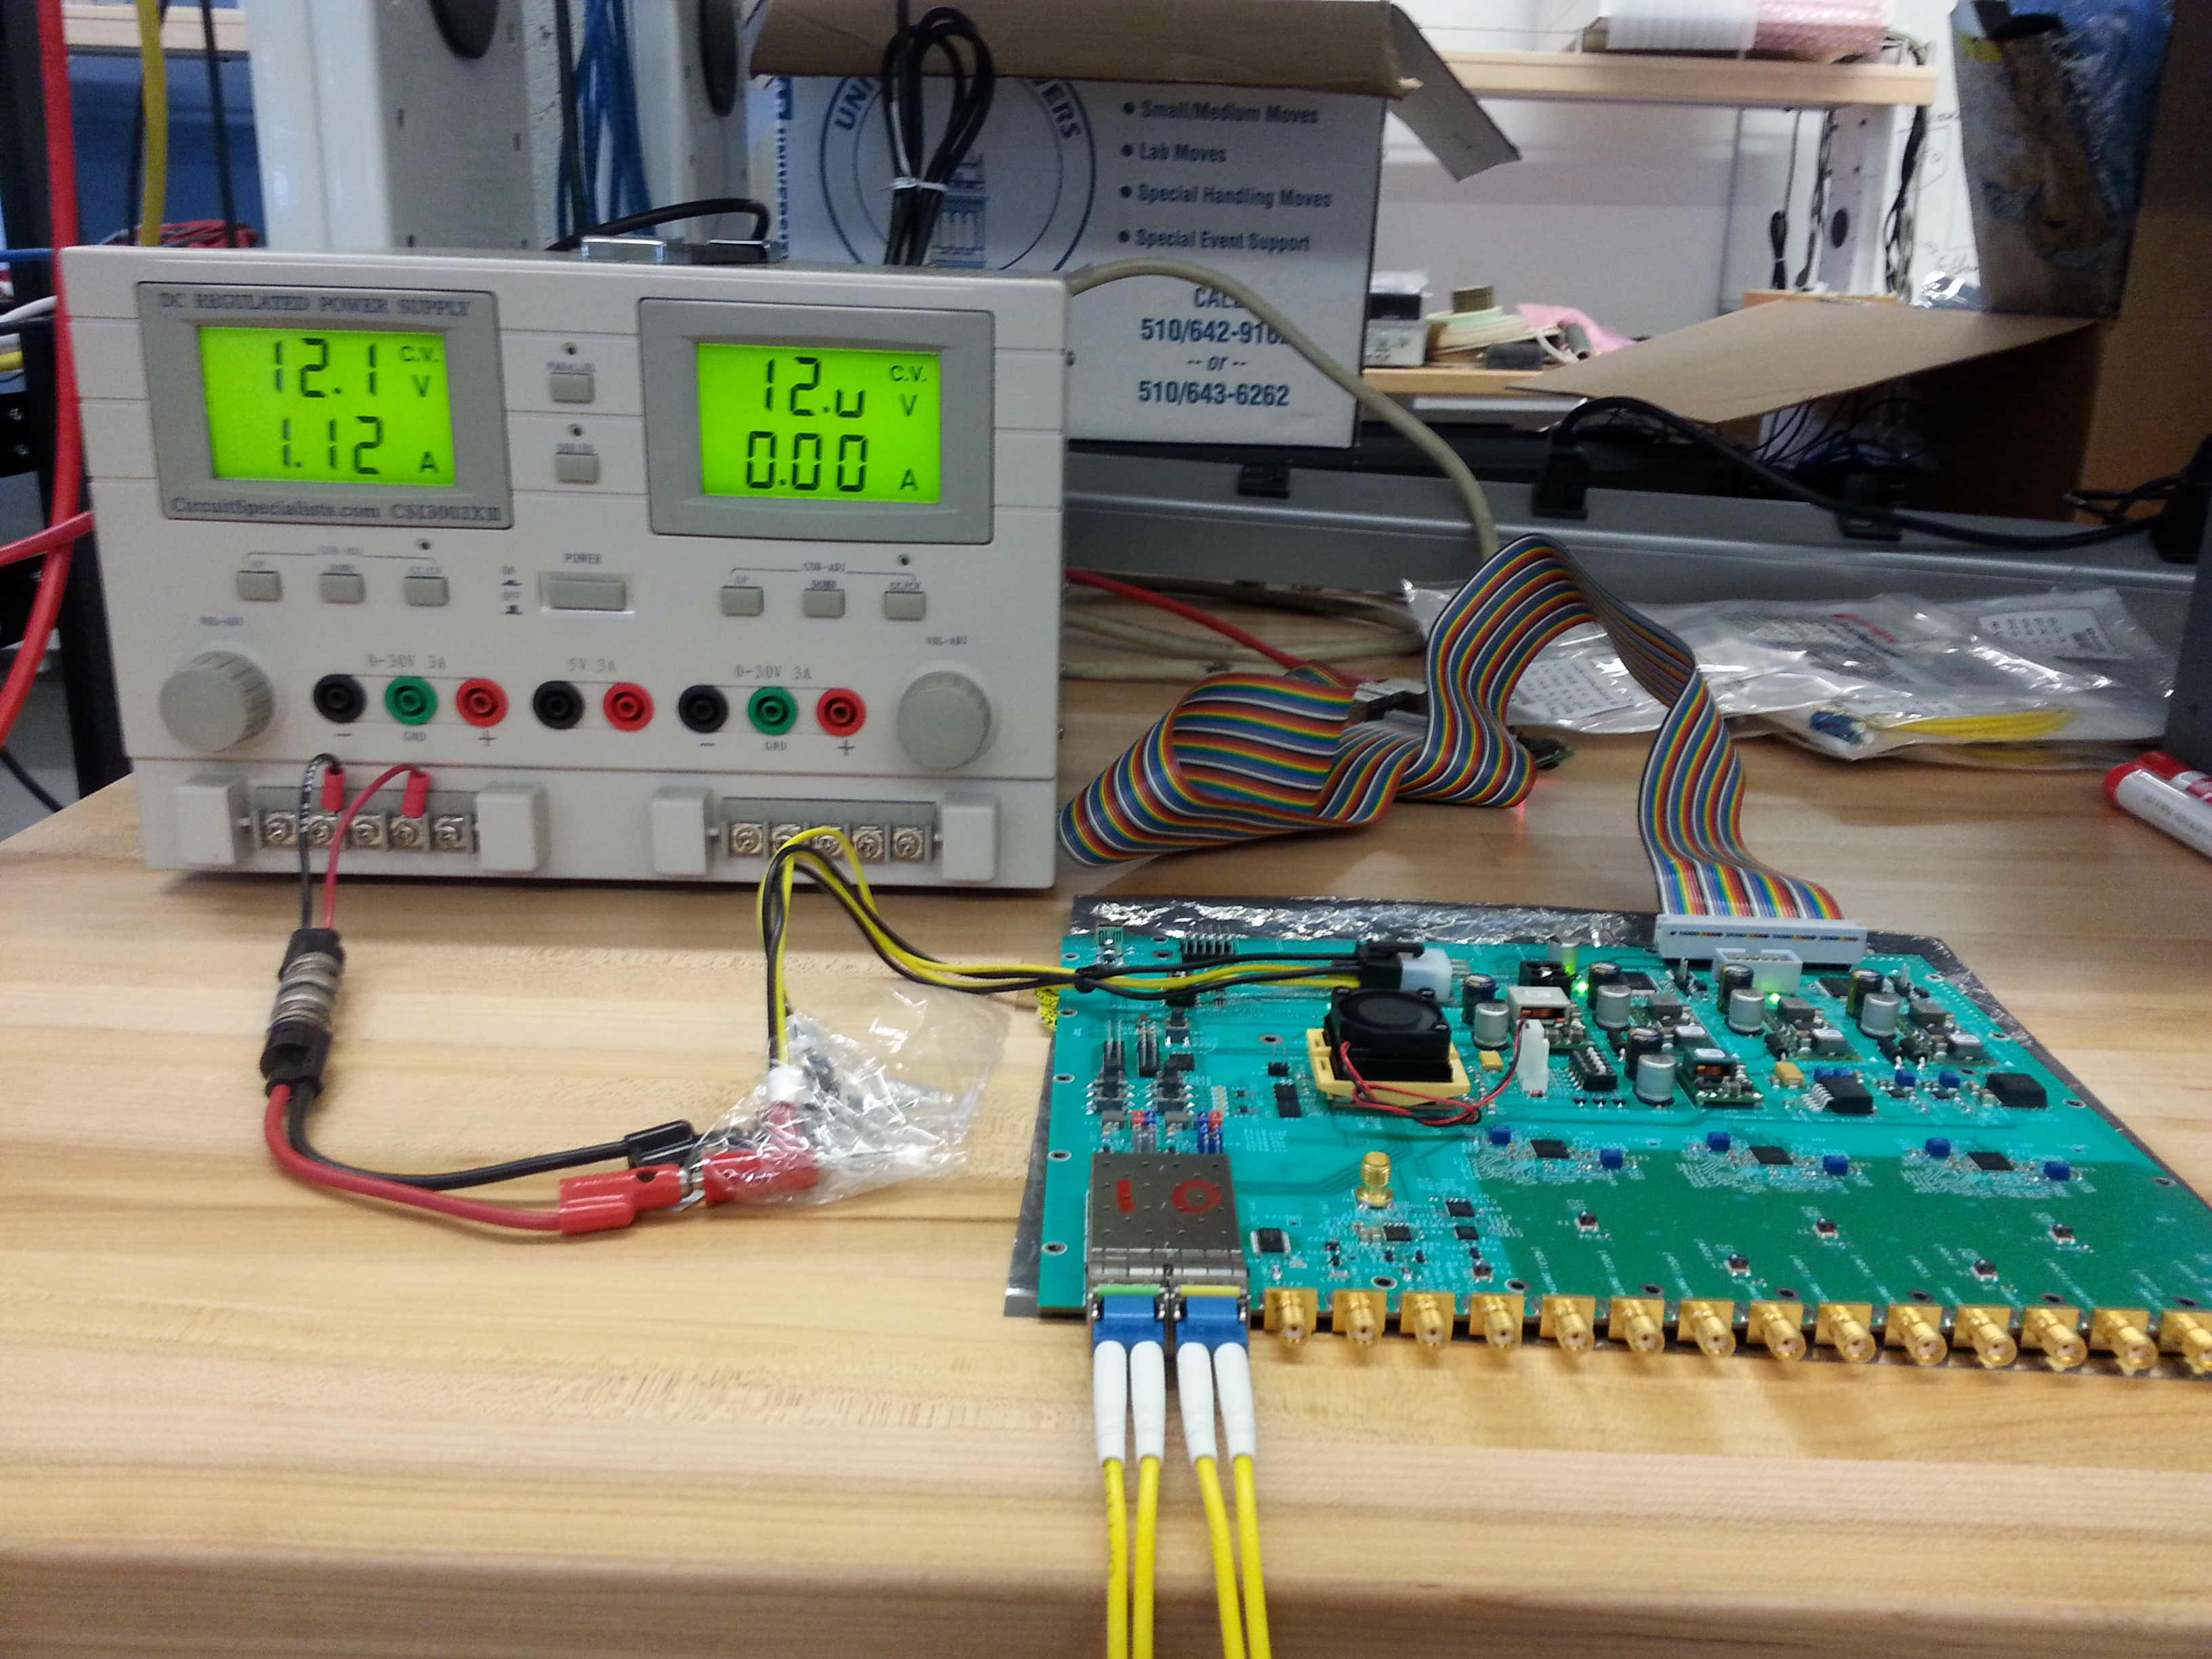
\includegraphics[width = .8\linewidth]{PowerSupply.png}
		\caption{Power Supply for SNAP board}
	\end{minipage}
\end{figure}

\section*{Software}
The boffile was loaded on raspberry pi attached to SNAP board via the python script:
\newline
python sfp\_test.py -b sfp2x\_test\_2015-6-30\_1458.bof -n 2 rpirachel -P 1000 -T 1100
\newline
Each data collection was executed at a wait period of 1100 clock cycles between packet transmissions(-T option). Since SNAP is running at 100MHz, the time between packet transmission is 1100/100e6 = 11 microseconds. The payload of each packet was specified to be 1000, which works out to be 8Kbytes since it is measured in 64 bit words(-P option). -n option selects the number of cores to be used on SNAP. More information could be found by running python sfp\_test.py -h command. The python script along with other files could be found on github: \url{https://github.com/reeveress/HERA-tests}.


\section*{Instrument Attenuations}

It is worthwhile to log the attenuations of various instruments involved. The power meter produces a 1310nm, 1KHz wave at -6.50dBm. 

\begin{center}
\begin{tabular}{|l|l|l|l|l|p{3cm}|}
	\hline
	Instrument & Attenuation & Optical Source & Power Meter reading\\ \hline
	Variable attenuator & 3.8dB & -6.50dBm & -10.3dBm\\ \hline
	LDNSTB & 5.6dB & -6.50dBm & -12.10dBm \\ \hline
\end{tabular}	
\end{center}
 

\section*{Power Tests}
\begin{center}
\begin{tabular}{|l|l|p{3cm}|}
	\hline
	 Transceiver type & Core 0  & Core 1 \\ \hline
	 pink & -2.2 dBm &  -2.2 dBm  \\ \hline
	 yellow & -0.4 dBm &  -0.5 dBm \\ \hline
	 blue & -2.0 dBm & -1.9 dBm\\ \hline
	 green & 0.4 dBm & 0.4 dBm \\ \hline
\end{tabular}
\end{center}



\section*{QSFP+ tests}
These tests used the 10GbE interface tutorial .bof file altered slightly to be used with a SNAP board. The design transmits noise over 10GbE from one SNAP core to another (the SNAP board we're using has core 0 and core 1). LC cables connect a transceivers' tx(transmit) outputs to the mux, the muxed COM fiber is then connected to the switch's QSFP+ transceiver, the QSFP+ is then routed to a demux and the rx (receive)of the respective SFP+ transceivers. The variable attenuator was placed either at the COM fiber going to the switch or the COM coming back from the switch to transceivers depending on the test. Note that each test also outputs bad crcs which are corrupted packets. Bad crcs value was zero for a successful test and one for a test with catastrophic packet loss. 
\begin{figure}[h]
\centering
	\begin{minipage}{.4\textwidth}
		\centering
		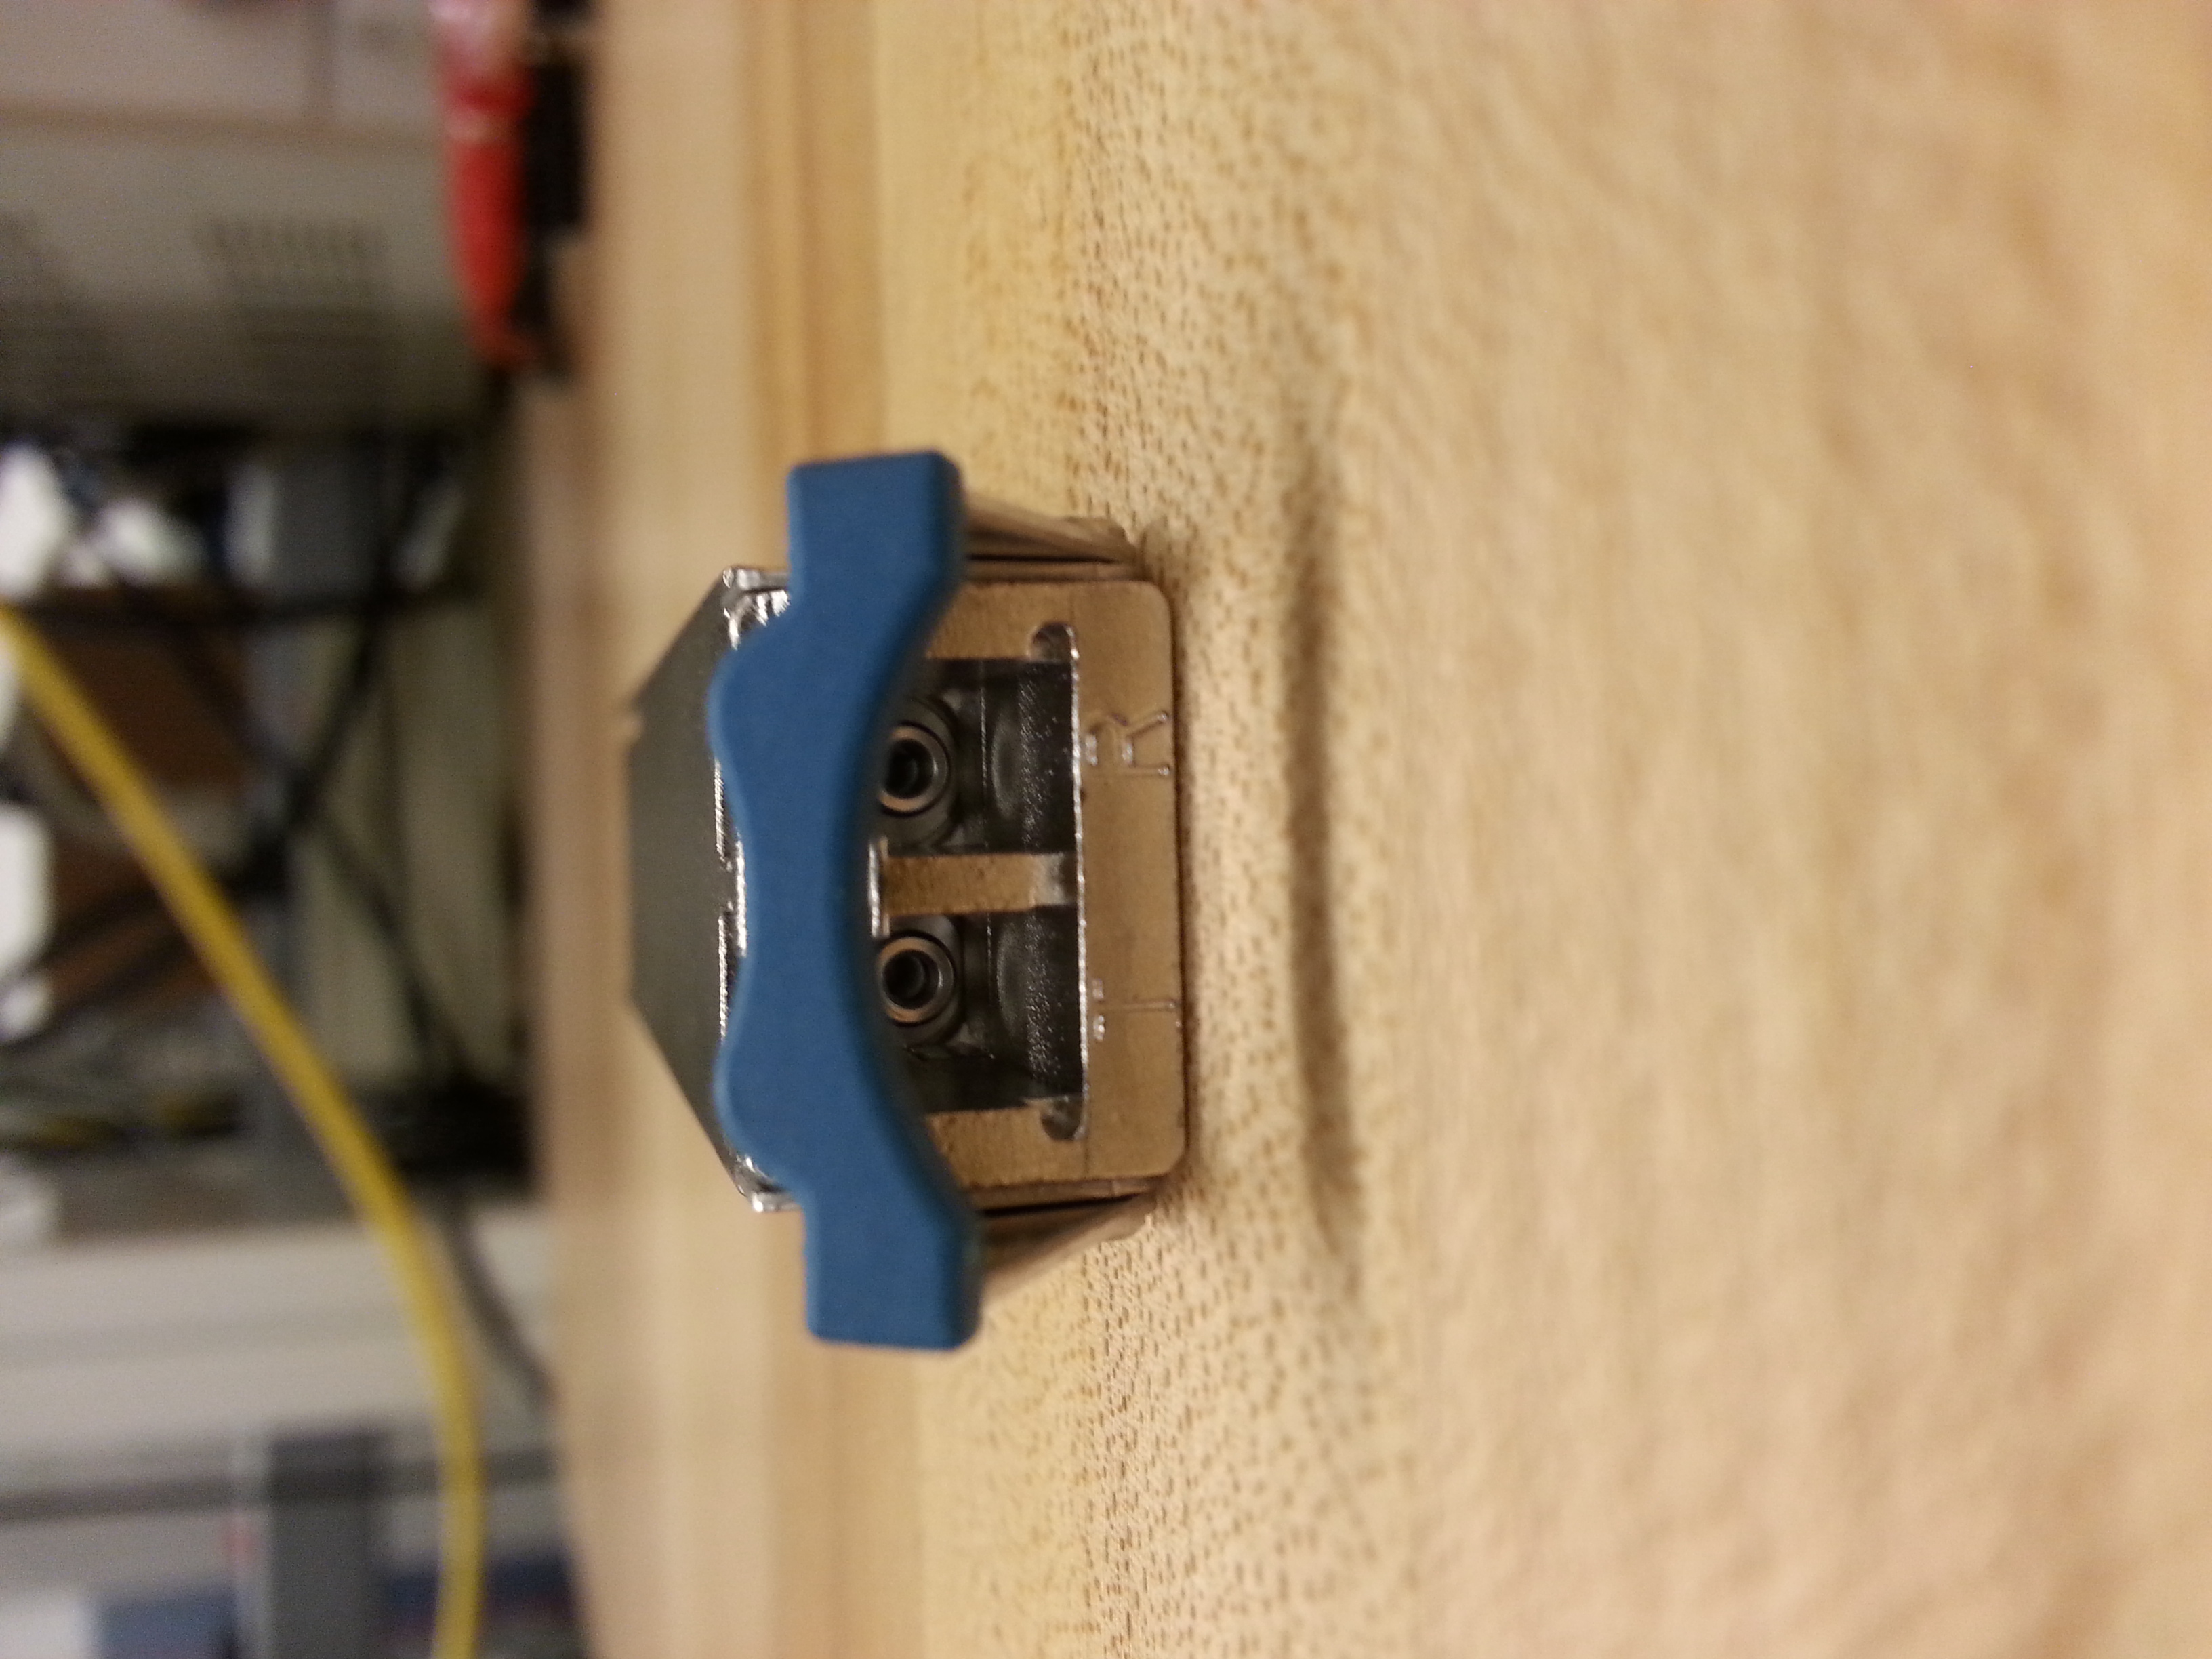
\includegraphics[width =.8\linewidth,height=2.6in]{qsfp.png}
		\caption{QSFP+ transceiver} 
	\end{minipage}
	\begin{minipage}{.4\textwidth}
		\centering
		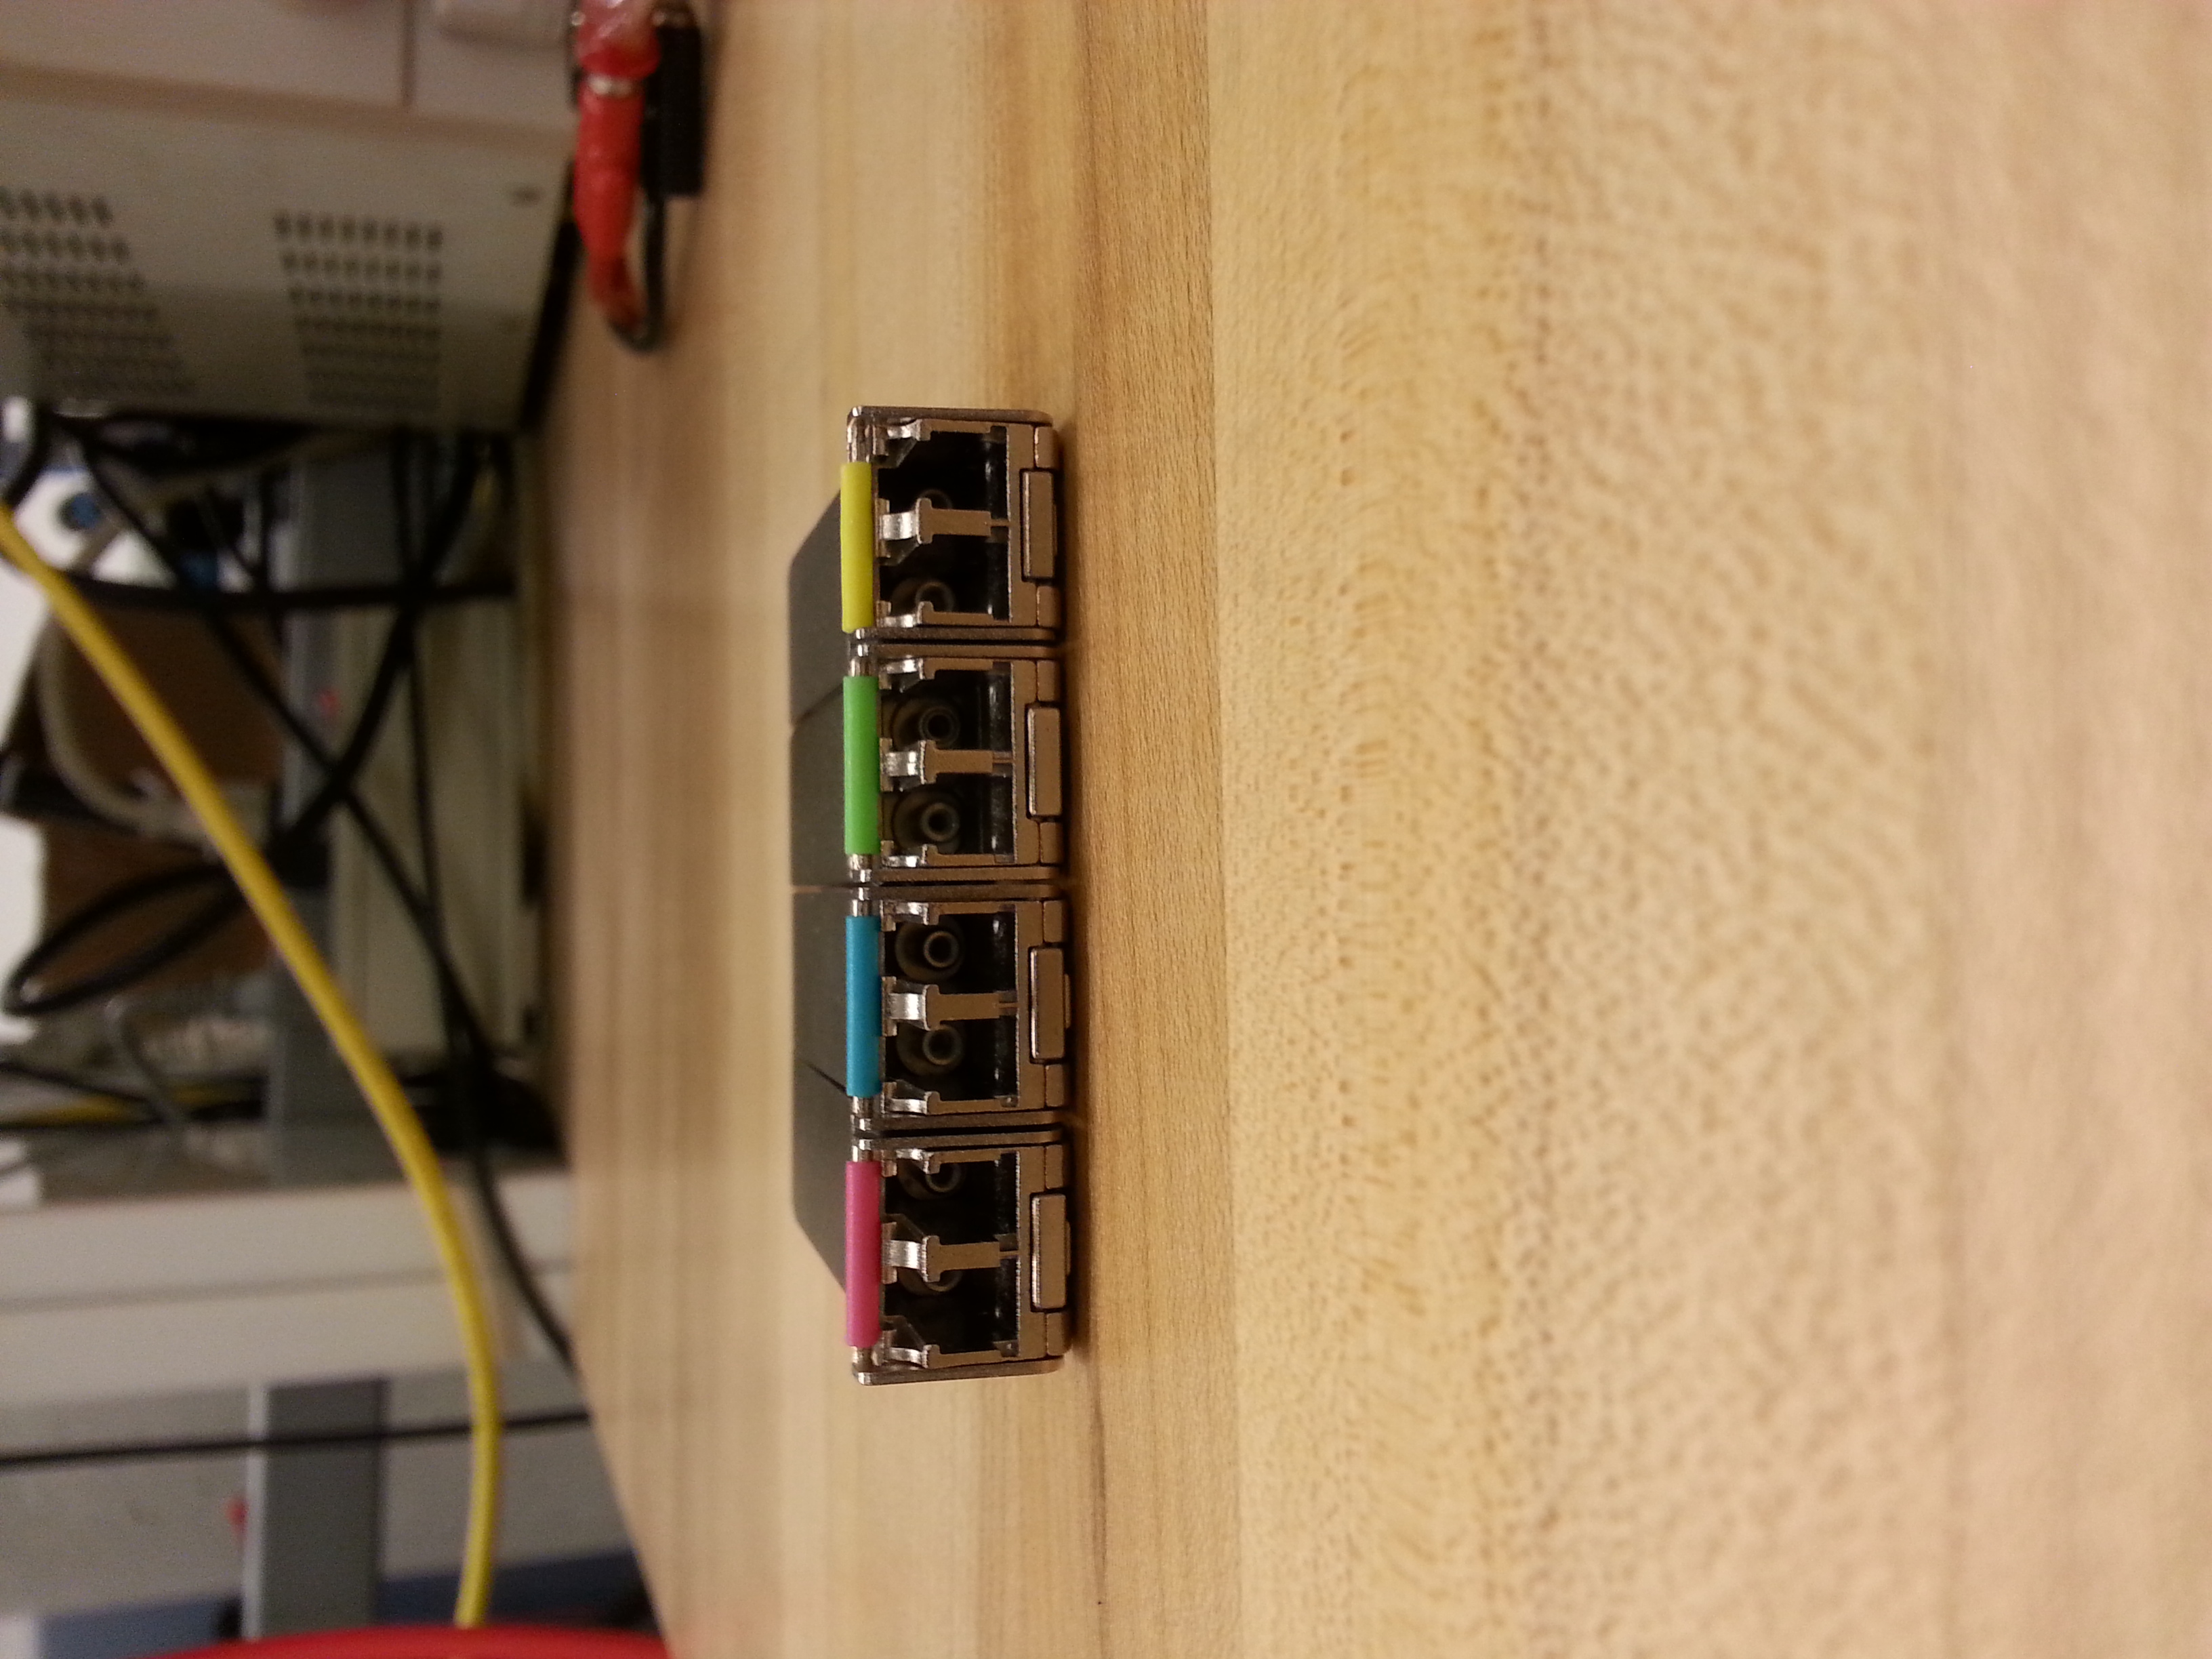
\includegraphics[width = .8\linewidth,height=2.6in]{sfp.png}
		\caption{SFP+ transceivers}
	\end{minipage}
\end{figure}

\clearpage
\afterpage{
\textbf{Test 1:}
Pink and Blue SFP+ transceivers were test with attenuator at the COM coming back from the switch as in Figure~\ref{fig:bluecore0} and Figure~\ref{fig:bluecore1}. The results are reported in Table~\ref{table:bluecore1} and Table ~\ref{table:bluecore0}.
\begin{figure}[h!]
	\begin{minipage}{.5\textwidth}
		\centering
		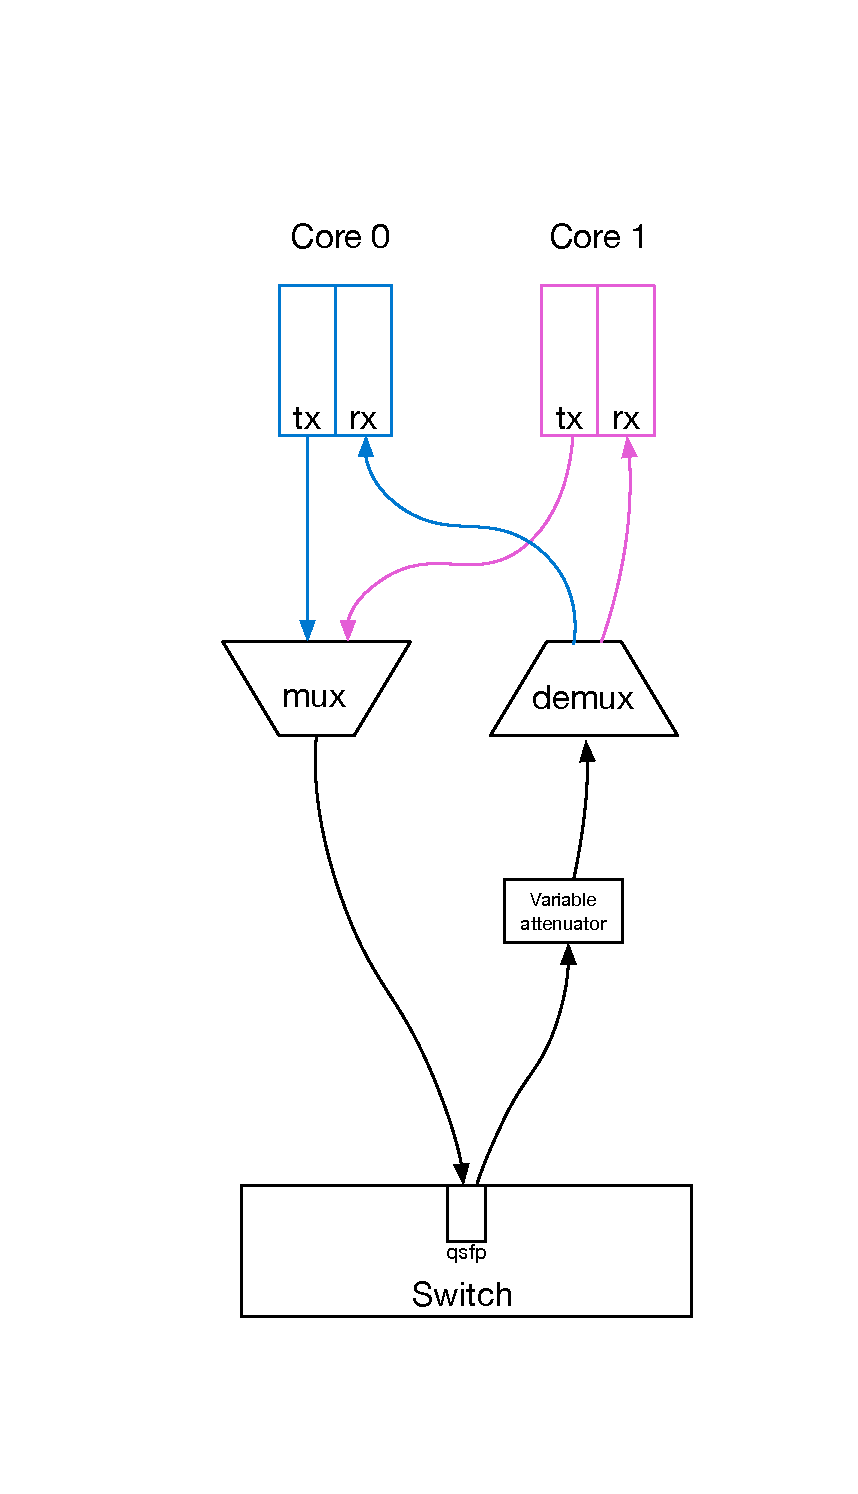
\includegraphics[width = .6\linewidth]{pinkbluecore0varrxcom.eps}
		\caption{Blue Core 0 , Pink Core 1}
		\label{fig:bluecore0}
	\end{minipage}
	\begin{minipage}{.5\textwidth}
		\centering
		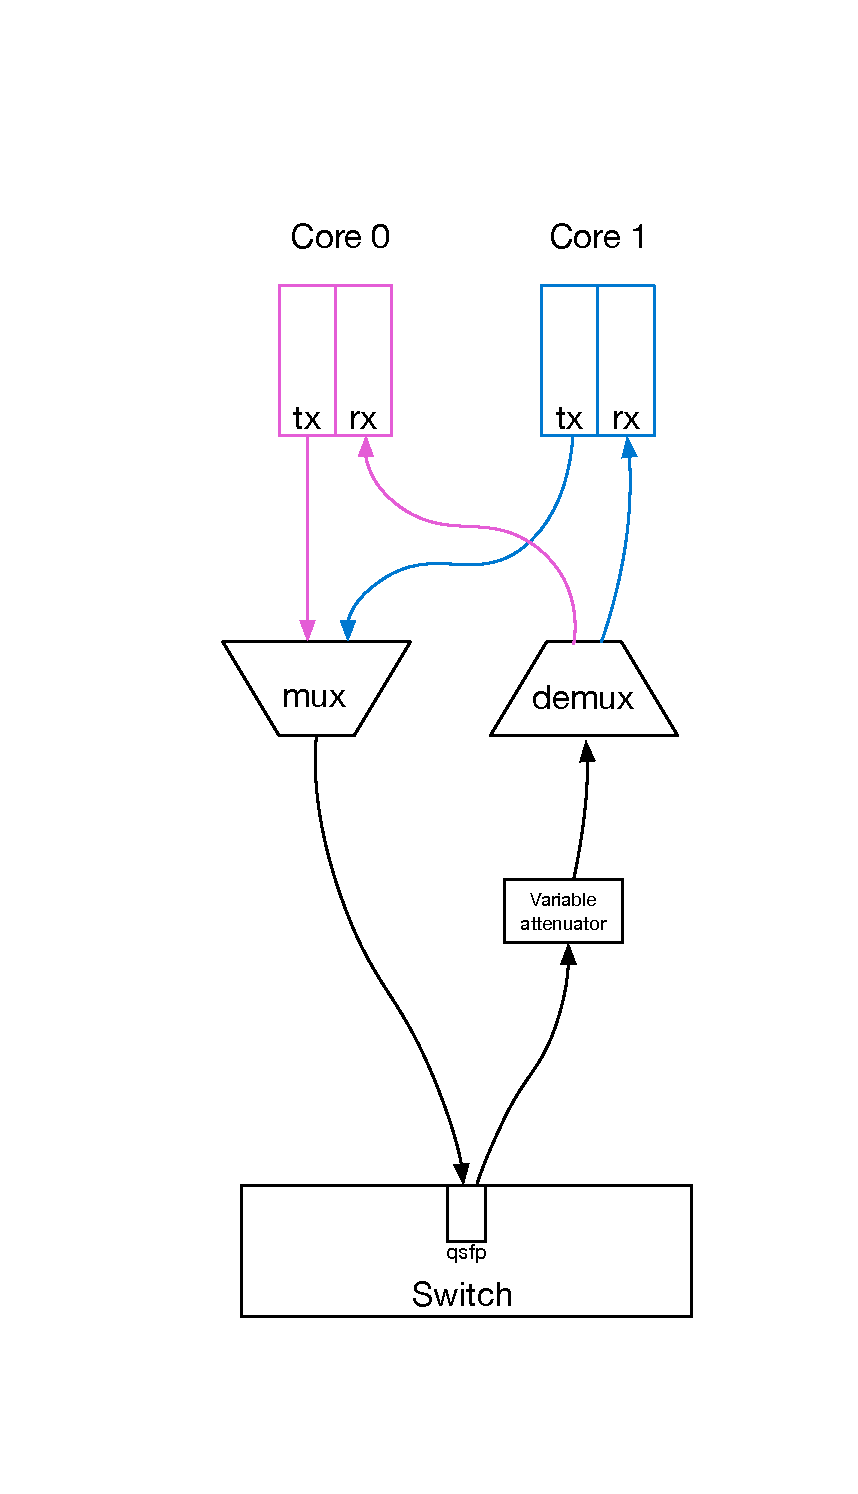
\includegraphics[width = .6\linewidth]{pinkbluecore1varrxcom.eps}
		\caption{Pink Core 0, Blue Core 1}
		\label{fig:bluecore1}
	\end{minipage}
\end{figure}

\begin{table}[ht]
\begin{minipage}{.5\textwidth}
\begin{center}
\begin{tabular}{|p{2.5cm}|p{2.5cm}|p{2.5cm}|}
	\hline
	 Attenuation(dB) & Duration(sec) & Packet loss \\ \hline
	 10 & 1000 & no packet loss \\ \hline
	 11 & 7800 & no packet loss \\ \hline
	 11.5 & 1000 & no packet loss \\ \hline
	 12 & 1000 &  catastrophic packet loss \\ \hline
\end{tabular}
\end{center}
\caption{Pink in Core 0, Blue in Core 1}
\label{table:bluecore1}
\end{minipage}
\begin{minipage}{.5\textwidth}
\begin{center}
\begin{tabular}{|p{2.5cm}|p{2.5cm}|p{2.5cm}|}
	\hline
	 Attenuation(dB) & Duration(sec) & Packet loss \\ \hline
	 10 & 1000 & no packet loss \\ \hline
	 11 & 7800 & no packet loss \\ \hline
	 11.5 & 1000 & catastrophic packet loss \\ \hline
\end{tabular}
\end{center}
\caption{Blue in Core 0 , Pink in Core 1}
\label{table:bluecore0}
\end{minipage}
\end{table}
}

\clearpage
\afterpage{
\textbf{Test 2:}
Similar tests were performed with yellow and green transceivers as in Figure~\ref{fig:greencore0} and Figure~\ref{fig:greencore1}.
The results are reported in Table~\ref{table:greencore0} and Table~\ref{table:greencore1}.
\begin{figure}[h!]
	\begin{minipage}{.5\textwidth}
		\centering
		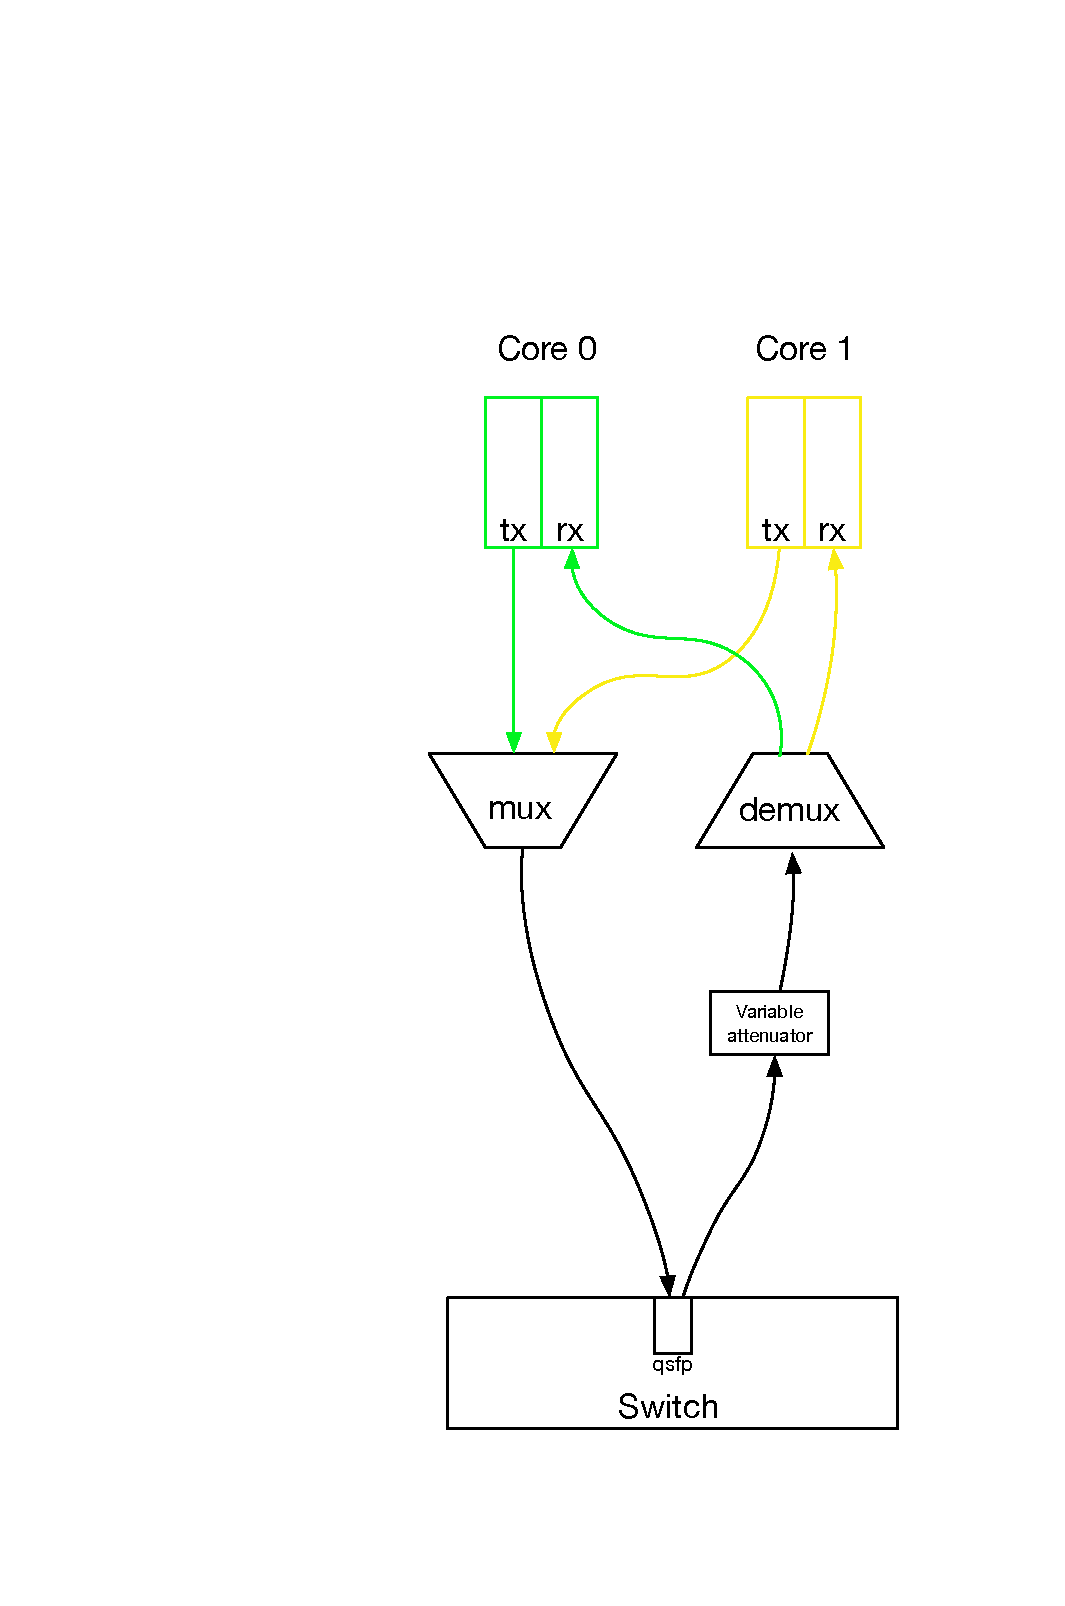
\includegraphics[width = .7\linewidth]{yellowgreencore0varrxcom.eps}
		\caption{Yellow in Core 0, Green in Core 1}
		\label{fig:greencore0}
	\end{minipage}
	\begin{minipage}{.5\textwidth}
		\centering
		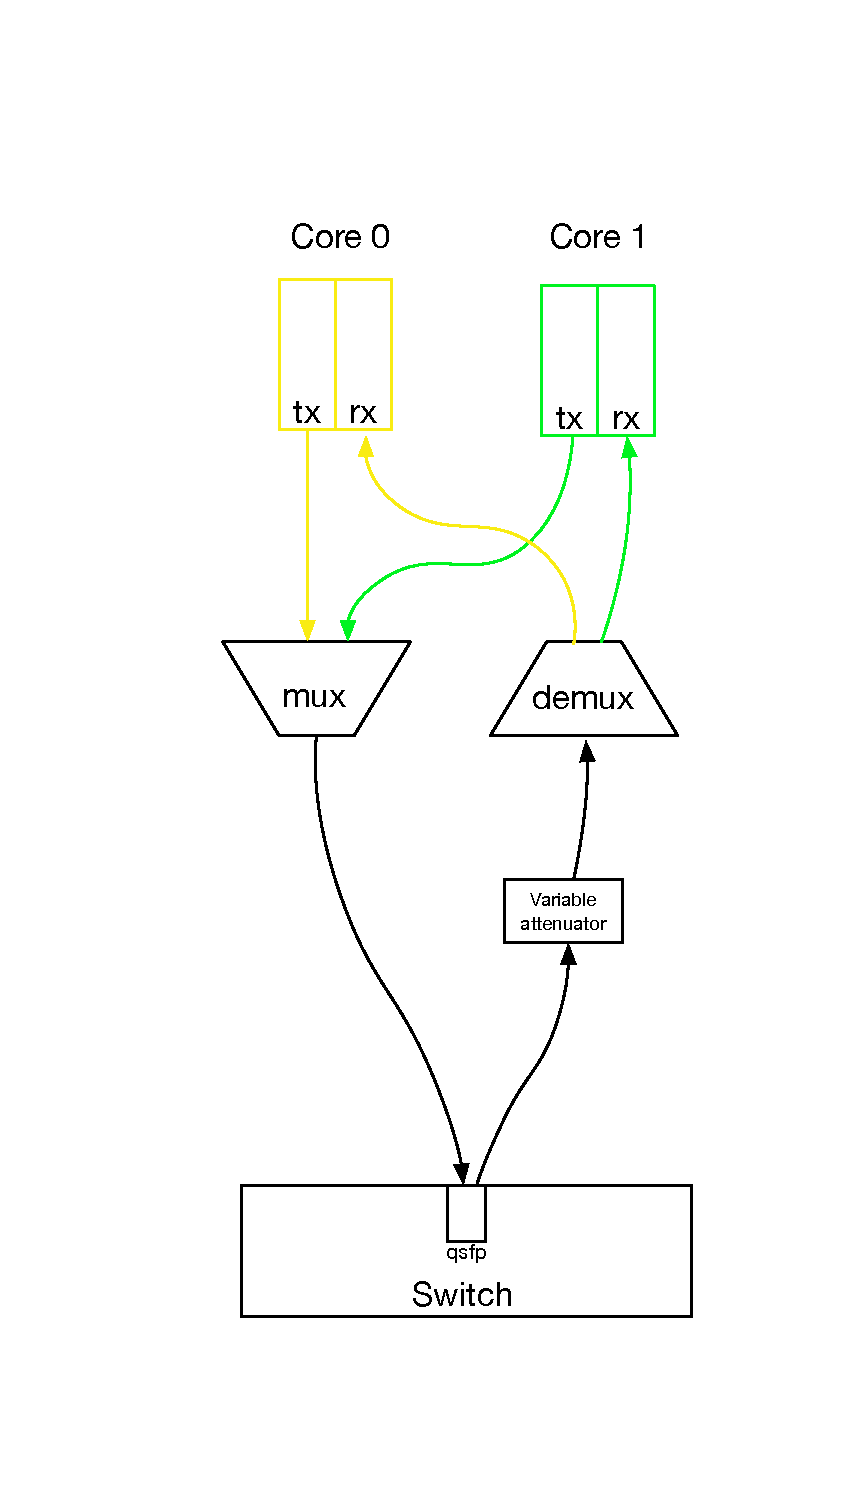
\includegraphics[width = .6\linewidth]{yellowgreencore1varrxcom.eps}
		\caption{Green in Core 0, Yellow in Core 1}
		\label{fig:greencore1}
	\end{minipage}
\end{figure}
\begin{table}[ht]
\begin{minipage}{.5\textwidth}
\begin{center}
\begin{tabular}{|p{2.5cm}|p{2.5cm}|p{2.5cm}|}
	\hline
	 Attenuation(dB) & Duration(sec) & Packet loss \\ \hline
	 7.5  & 3000 &  no packet loss \\ \hline
	 8.0  &  2000 & catastrophic packet loss \\ \hline
	 8.5  & 1500 & catastrophic packet loss \\ \hline
\end{tabular}
\end{center}
\caption{Yellow in Core 0, Green in Core 1}
\label{table:greencore1}
\end{minipage}
\begin{minipage}{.5\textwidth}
\begin{center}
\begin{tabular}{|p{2.5cm}|p{2.5cm}|p{2.5cm}|}
	\hline
	 Attenuation(dB) & Duration(sec) & Packet loss \\ \hline
	 7.5  & 3000 &  no packet loss \\ \hline
	 8.0  &  1200 & no packet loss \\ \hline
	 8.5  & 1000 & no packet loss \\ \hline
	 9.0  & 300 & catastrophic packet loss \\ \hline
\end{tabular}
\end{center}
\caption{Green in Core 0, Yellow in Core 1}
\label{table:greencore0}
\end{minipage}
\end{table}
}



\clearpage
\textbf{Test 3:}
It was also imported to test the link margin of the SFP+ transceivers. Thus the attenuator was placed at the COM fiber going from SNAP to the switch as in Figure~\ref{fig:pinkcore1} and Figure~\ref{fig:pinkcore0}. Test results are reported in Table~\ref{table:pinkcore1} and Table~\ref{table:pinkcore0}.
\afterpage{
\begin{figure}[h!]
	\begin{minipage}{.5\textwidth}
		\centering
		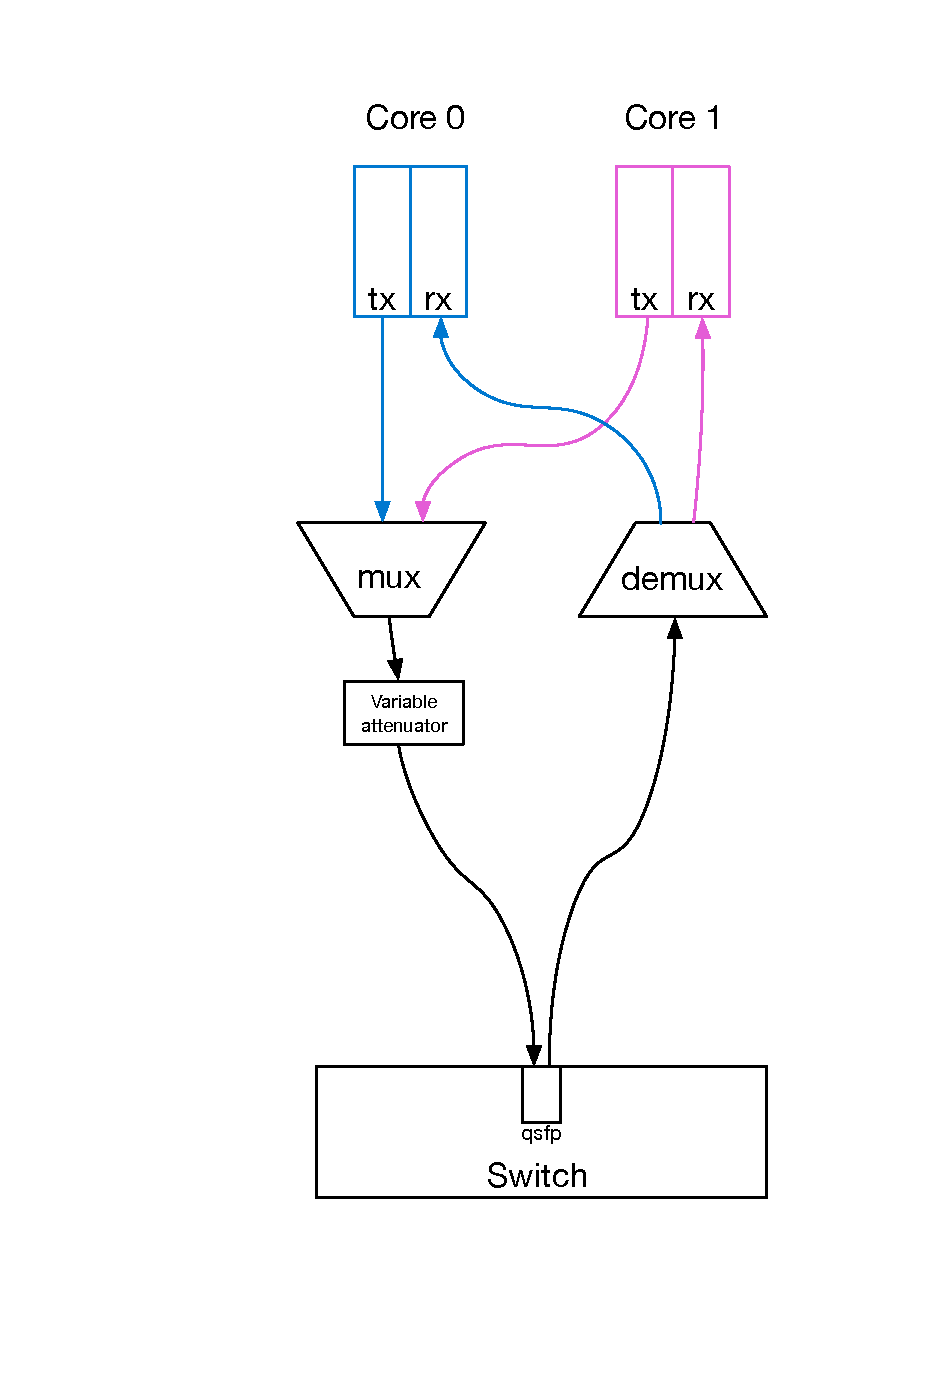
\includegraphics[width = .6\linewidth]{pinkbluecore0vartxcom.eps}
		\caption{Blue in Core 0, Pink in Core 1}
		\label{fig:pinkcore1}
	\end{minipage}
	\begin{minipage}{.5\textwidth}
		\centering
		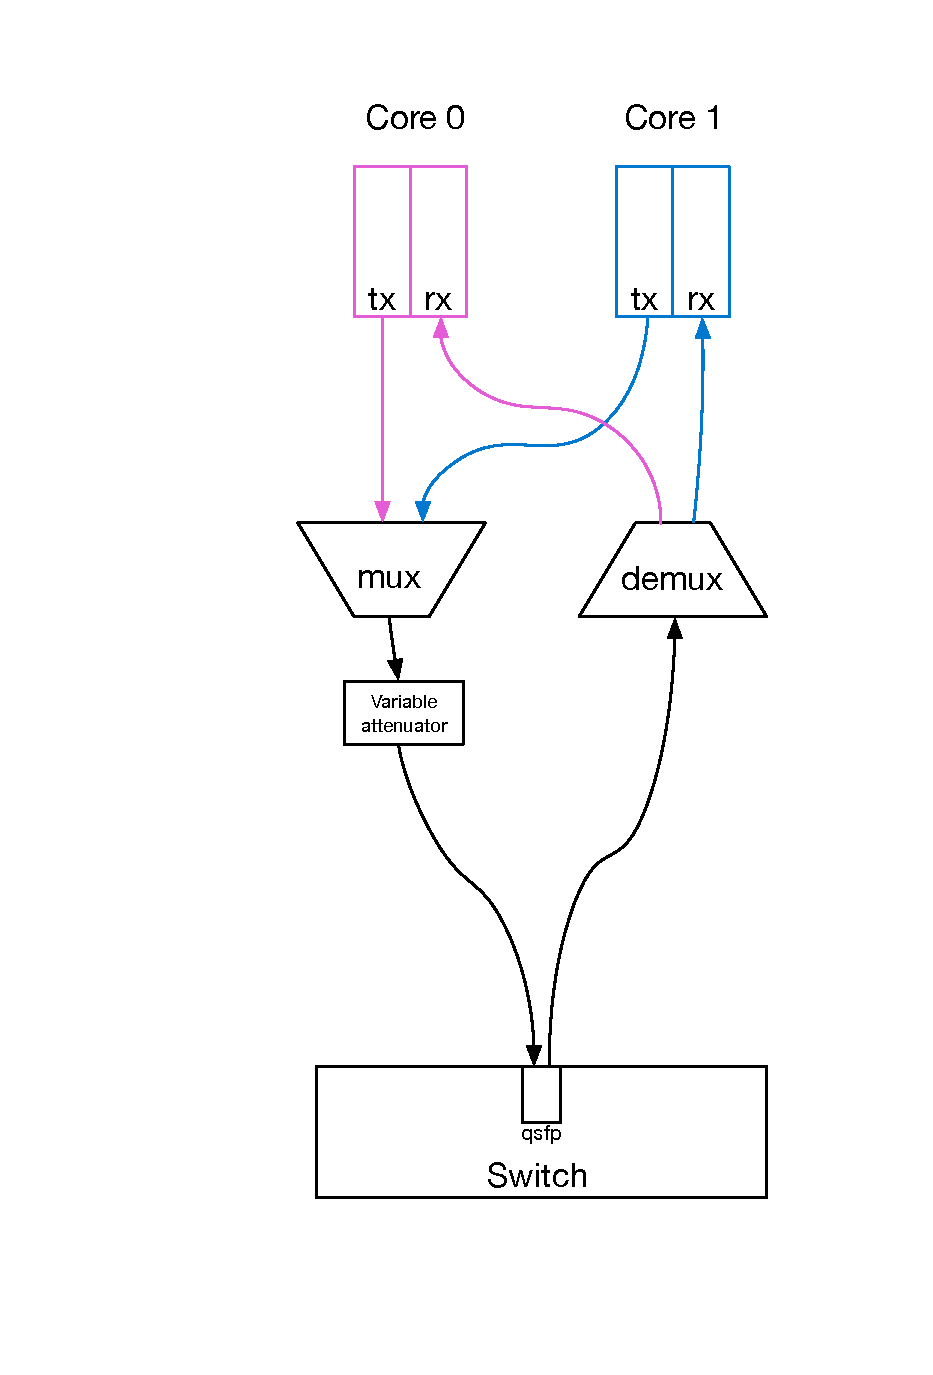
\includegraphics[width = .6\linewidth]{pinkbluecore1vartxcom.eps}
		\caption{Pink in Core 0, Blue in Core 1}
		\label{fig:pinkcore0}
	\end{minipage}
\end{figure}
\begin{table}[ht]
\begin{minipage}{.5\textwidth}
\begin{center}
\begin{tabular}{|p{2.5cm}|p{2.5cm}|p{2.5cm}|}
	\hline
	 Attenuation(dB) & Duration(sec) & Packet loss \\ \hline
         7.0  & 1000 & no packet loss \\ \hline
	 7.5 & 1000 & catastrophic packet loss \\ \hline
	 8.0  &  200 & catastrophic packet loss \\ \hline
\end{tabular}
\end{center}
\caption{Blue in Core 0, Pink in Core 1}
\label{table:pinkcore1}
\end{minipage}
\begin{minipage}{.5\textwidth}
\begin{center}
\begin{tabular}{|p{2.5cm}|p{2.5cm}|p{2.5cm}|}
	\hline
	 Attenuation(dB) & Duration(sec) & Packet loss \\ \hline
	 7.0  & 1000 & no packet loss \\ \hline
	 7.5 & 1000 & no packet loss \\ \hline
	 8.0  &  200 & catastrophic packet loss \\ \hline
\end{tabular}
\end{center}
\caption{Pink in Core 0, Blue in Core 1}
\label{table:pinkcore0}
\end{minipage}
\end{table}
}

\clearpage
\afterpage{
\textbf{Test 4:}
Similar tests were done with the yellow and green transceivers, attenuator on the COM fiber going towards Arista switch as in Figure~\ref{fig:yellowcore1} and Figure~\ref{fig:yellowcore0}. Test results are reported in Table~\ref{table:yellowcore1} and Table~\ref{table:yellowcore0}.
\begin{figure}[h!]
	\begin{minipage}{.5\textwidth}
		\centering
		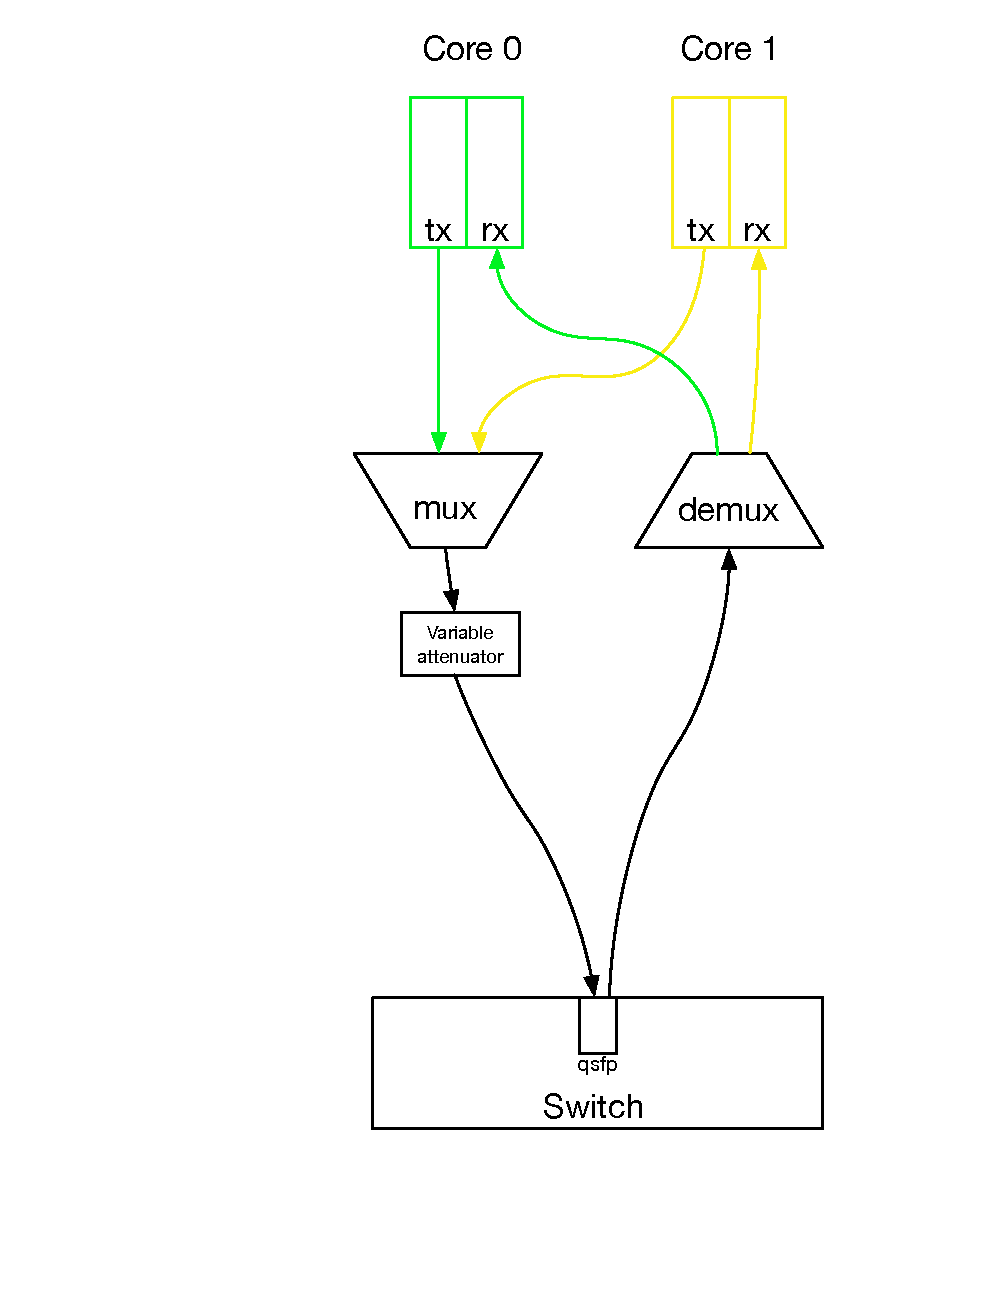
\includegraphics[width = .6\linewidth]{yellowgreencore0vartxcom.eps}
		\caption{Green in Core 0, Yellow in Core 1}
		\label{fig:yellowcore1}
	\end{minipage}
	\begin{minipage}{.5\textwidth}
		\centering
		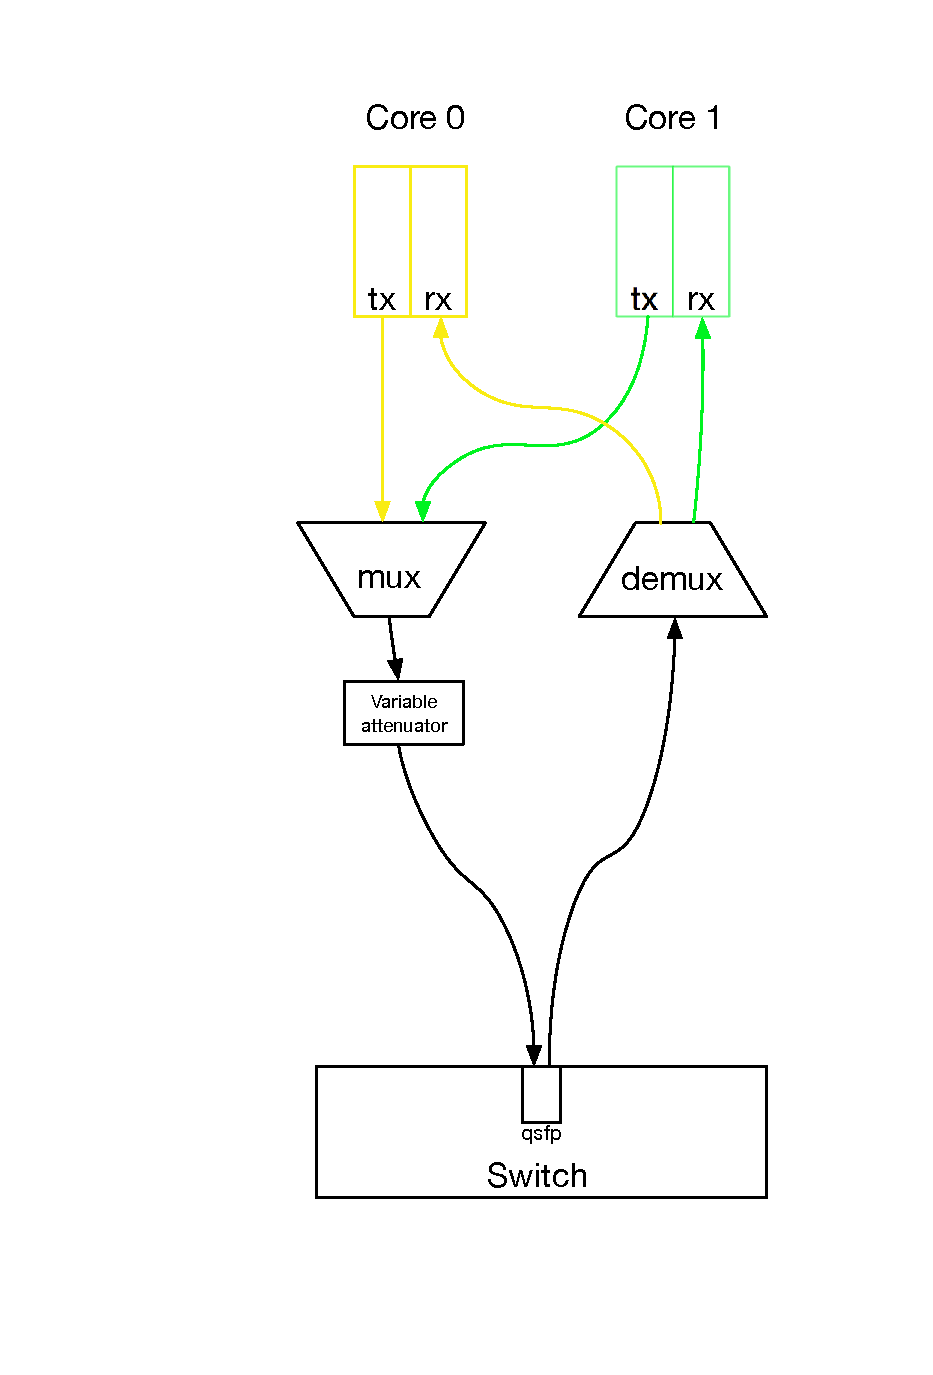
\includegraphics[width = .6\linewidth]{yellowgreencore1vartxcom.eps}
		\caption{Yellow in Core 0 , Green in Core 1}
		\label{fig:yellowcore0}
	\end{minipage}
\end{figure}
\begin{table}[ht]
\begin{minipage}{.5\textwidth}
\begin{center}
\begin{tabular}{|p{2.5cm}|p{2.5cm}|p{2.5cm}|}
	\hline
	 Attenuation(dB) & Duration(sec) & Packet loss \\ \hline
	 8.0  &  6000 & no packet loss \\ \hline
	 8.5  & 1000 & catastrophic packet loss \\ \hline
\end{tabular}
\end{center}
\caption{Green in Core 0, Yellow in Core 1}
\label{table:yellowcore1}
\end{minipage}
\begin{minipage}{.5\textwidth}
\begin{center}
\begin{tabular}{|p{2.5cm}|p{2.5cm}|p{2.5cm}|}
	\hline
	 Attenuation(dB) & Duration(sec) & Packet loss \\ \hline
	 8.0  &  2000 & no packet loss \\ \hline
	 8.5  & 900 & catastrophic packet loss \\ \hline
\end{tabular}
\end{center}
\caption{Yellow in Core 0 , Green in Core 1}
\label{table:yellowcore0}
\end{minipage}
\end{table}
}

\section*{Conclusion}
The link margin of SFP+ and QSFP+ transceiver system is about 7.5dB + the inherent attenuation of the attenuator(~3.8dB) = 11.3dB. The 10km spool of fiber is about 5.6dB thus this margin should be sufficient for the data transport required for HERA. 

\section*{References}
Steenbergen, Richard A. \it{Everything You Always Wanted to Know About Optical Networking - But Were Afraid to Ask}. N.p.: Nanog.org, Feb. 2013. PDF.
"Fiber Optic Basics."  \it {Newport Corporation} .N.p., n.d. Web. http://www.newport.com/Fiber-Optic-Basics/978863/1033/content.aspx

Steenbergen, Richard A. "Everything You Always Wanted to Know About Optical Networking ? But Were Afraid to Ask." \it{The New Schelling} (2004): n. pag. Web. https://www.nanog.org/meetings/nanog57/presentations/Monday/mon.tutorial.Steenbergen.Optical.39.pdf.


\end{document} 
